%%% EventSelection %%%

%%This section describes the event selection, which has been optimized in order to maximize the expected significance of the signal over background.
%%
%%A set of preselection cuts are applied first, including basic quality cuts (event cleaning) and  trigger requirements.
%%Some preselection cuts applied in the \texttt{CxAODMaker} are also summarized.

This chapter outlines the event selection process, optimized to enhance the expected significance of the signal relative to the background.
A series of preselection criteria are employed, including basic quality cuts (event cleaning) and trigger requirements. Additionally, the preselection cuts applied in the \texttt{CxAODMaker} are outlined.

In the primary phase of event selection, the focus is on identifying the $W/Z$ boson decaying leptonically. For the 1-lepton channel, the candidate boson is chosen targeting $W\to \ell\nu$.
Next, the focus shifts to the hadronic components of the final state. This step aims to enhance the identification of VBS-associated objects and to select the (second) boson that decays hadronically. For selecting VBS-jet candidates, a standard tagging jets procedure is implemented. The hadronically decaying $V$ candidate is identified, either as a large-$R$ jet in the merged regime or as a pair of small-$R$ jets in the resolved regime. 

After the two bosons are indentified, topological cuts are applied to further reduce the background. In the merged regime, the boson tagger defines the SRs and a reversed cut specifies CRs for the \Vjets background. In the resolved regime, a signal di-jets system is constructed, and its invariant mass is utilized to deine a mass window for SRs or sidebands for \Vjets CRs. Additionally, for the \olep channel, dedicated TopCRs are established by including events with additional b-jets.

%The next section concludes with a summary of all the selections, offering a comprehensive overview to the reader. Following this, the chapter will delve into detailed explanations of each selection.

The selections applied are summarized here in tables
\ref{tab:1lep_merged}-\ref{tab:1lep_resolved}
.
%Following this, the current chapter will delve into detailed explanations of each selection.
Subsequent sections of this chapter will provide detailed discussions of each selection criterion, following the sequence in which they were applied.

%%% 1-lepton channel
\begin{table}[t]
\caption{A summary of regions event selection for \olep channel in the merged regime.}
\label{tab:1lep_merged}
\begin{center}
\resizebox{\textwidth}{!}{
\begin{tabular}{|l|l|c|c|c|c|c|}
\hline
\multicolumn{2}{|l|}{\multirow{2}{*}{Selection}} & \multicolumn{2}{c|}{SR}  &  $W$ CR (WR)  & \multicolumn{2}{c|}{$t\bar{t}$ CR (TR)} \\
\cline{3-7}
\multicolumn{2}{|l|}{} & HP & LP & incl & HP & LP \\
\hline
\multirow{4}{*}{$W\rightarrow \ell\nu$} & Num of Tight leptons & \multicolumn{5}{c|}{ 1 } \\
\cline{2-7}
&Num of Loose (!Tight) leptons & \multicolumn{5}{c|}{ 0 }  \\
\cline{2-7}
&\vphantom{\Large B} \met & \multicolumn{5}{c|}{ $>80\,\si{\GeV}$ } \\
\cline{2-7}
&\pt{$(\ell)$} & \multicolumn{5}{c|}{ $>28\,\si{\GeV}$ } \\
\hline
\multirow{3}{*}{VBS jets candidates} & Leading Tag jet \pt & \multicolumn{5}{c|}{ $>30\,\si{\GeV}$ } \\
\cline{2-7}
                          & Subleading Tag jet \pt & \multicolumn{5}{c|}{ $>30\,\si{\GeV}$ }\\
\cline{2-7}
                          & $m_{jj}$ & \multicolumn{5}{c|}{ $> 400 \si{\GeV}$ } \\
\hline
\multirow{2}{*}{$W/Z\rightarrow J$} & Num of large-$R$ jets & \multicolumn{5}{c|}{ $\geq 1$ } \\
\cline{2-7}
& 3-Var Tagger & pass50WP & pass80WP \&\& !pass50WP & fail80WP & pass50WP & pass80WP \&\& !pass50WP \\
%& \vphantom{\Large B} $D_2/n_{Tracks}$ cut & pass & fail & pass & fail & pass & fail \\
%\cline{2-8}
%& $W/Z$ mass window cut & pass & pass & fail & fail & pass & pass\\
\hline
Top veto & Num of $b$-tagged jets outside of large-R jet & \multicolumn{3}{c|}{0} & \multicolumn{2}{c|}{$\geq 1$} \\
\hline
\end{tabular}
}
\end{center}
\end{table}

\begin{table}[t]
  \caption{A summary of regions event selection for \olep channel in the resolved regime.}
\label{tab:1lep_resolved}
\begin{center}
\resizebox{\textwidth}{!}{
\begin{tabular}{|l|l|c|c|c|}
\hline
\multicolumn{2}{|l|}{Selection} & SR & $W$ CR (WR) & \ttbar CR (TR) \\
\hline
\multirow{4}{*}{$W\rightarrow \ell\nu$ } & Number of Tight leptons & \multicolumn{3}{c|}{ 1 } \\
\cline{2-5}
&Number of Loose (!Tight) leptons & \multicolumn{3}{c|}{ 0 }  \\
\cline{2-5}
&\met & \multicolumn{3}{c|}{ $>80\,\si{\GeV}$ } \\
\cline{2-5}
&\pt{$(\ell)$} & \multicolumn{3}{c|}{ $>28\,\si{\GeV}$ } \\
\hline
\multirow{3}{*}{VBS jets candidates} & Leading Tag jet \pt & \multicolumn{3}{c|}{ $>30\,\si{\GeV}$ } \\
\cline{2-5}
                          & Subleading Tag jet \pt & \multicolumn{3}{c|}{ $>30\,\si{\GeV}$ }\\
\cline{2-5}
                          & $m_{jj}$ & \multicolumn{3}{c|}{ $> 400 \si{\GeV}$ } \\
\hline
\multirow{4}{*}{$W/Z\rightarrow jj$ } & Number of small-R jets & \multicolumn{3}{c|}{ $\geq 4$ } \\ %$\geq 2$ & $\geq 2$ & $\geq 2$  \\
\cline{2-5}
& Leading jet \pt & \multicolumn{3}{c|}{ $>40\,\si{\GeV}$}\\
\cline{2-5}
& Subleading jet \pt & \multicolumn{3}{c|}{ $>20\,\si{\GeV}$}\\
\cline{2-5}
 &$Z \to q\bar{q}$ and $W \to qq'$     &   $64 < m_{jj} < 106 \, \si{\GeV}$ & $50<m_{jj}<64 \, \si{\GeV}$ or $m_{jj}>106 \, \si{\GeV} $ & $64 < m_{jj} < 106 \, \si{\GeV}$ \\
\hline
Top veto &  Number of additional $b$-tagged jets & \multicolumn{2}{c|}{0} & $\geq 1$ \\
\hline
VBS enhancing & $m_{jjj}$ & \multicolumn{3}{c|}{ $>220\,\si{\GeV}$} \\
\hline
\end{tabular}
}
\end{center}
\end{table}


%%% move here after Oldrich comment
%%\clearpage
\subsection{Summary of the SR and CR selections}
\label{subsec:summary_selection}

The selections applied are summarized here in tables 
\ref{tab:0lep_merged}-\ref{tab:0lep_resolved}
\ref{tab:1lep_merged}-\ref{tab:1lep_resolved}
\ref{tab:2lep_merged}-\ref{tab:2lep_resolved}
.

In particular, only the Tight selection is shown for the resolved regime in the relevant tables; 
the loose resolved selection (w/o $M_{jjj}$ cut) has been used only for validation and not for the final results.

%%% 0-lepton channel
\begin{table}[ht!]
\small
\caption{A summary of regions event selection for \zlep channel in the merged regime.}
\label{tab:0lep_merged}
\begin{center}
\resizebox{\textwidth}{!}{
\begin{tabular}{|l|l|c|c|c|}
\hline
\multicolumn{2}{|l|}{\multirow{2}{*}{Selection}} & \multicolumn{2}{c|}{SR}  &  $V$ CR \\
\cline{3-5}
\multicolumn{2}{|l|}{} & HP & LP &  \\
\hline
\multirow{3}{*}{$Z \to \nu\nu$}  &  Number of Loose leptons & \multicolumn{3}{c|}{0} \\
\cline{2-5}
    & \met                                     & \multicolumn{3}{c|}{ > 200 GeV }                  \\
\cline{2-5}
    & \mpt                                     & \multicolumn{3}{c|}{ > 50 GeV}                    \\
\hline

\multirow{3}{*}{anti-QCD}  & min($\Delta\Phi$(\met,small-R jets))     & \multicolumn{3}{c|}{ $> \pi/6$} \\
\cline{2-5}
    & $\Delta\Phi$(\met,\mpt)                  & \multicolumn{3}{c|}{ $< \pi/2$}                   \\
\cline{2-5}
    & $\Delta\phi(\met, Sig-J)$                & \multicolumn{3}{c|}{ $> \pi/9$}                   \\
\hline
\multirow{3}{*}{VBS jets candidates} & Leading Tag jet \pt & \multicolumn{3}{c|}{ $>30\,\GeV$ } \\
\cline{2-5}
                          & Subleading Tag jet \pt & \multicolumn{3}{c|}{ $>30\,\GeV$ }\\
\cline{2-5}
                          & $m_{jj}$ & \multicolumn{3}{c|}{ $> 400 \GeV$ } \\
\hline
\multirow{2}{*}{$W/Z \to J$} & Num of large-R jets & \multicolumn{3}{c|}{$\geq 1$} \\
\cline{2-5}
& 3-Var Tagger & pass50WP & pass80WP \&\& !pass50WP & fail80WP \\
%($W/Z$ mass window, $D_2$, $n_{Tracks}$ cuts)} 
%& \vphantom{\Large B} $D_2/n_{Tracks}$ cut & pass & fail & pass & fail \\
%\cline{2-6}
%& $W/Z$ mass window cut & pass & pass & fail & fail \\
%& \\
\hline
\end{tabular}
}
\end{center}
\end{table}




\begin{table}[ht!]
\small
\caption{A summary of regions event selection for \zlep channel in the resolved regime.}
\label{tab:0lep_resolved}
\begin{center}
\resizebox{\textwidth}{!}{
\begin{tabular}{|l|l|c|c|}
\hline
\multicolumn{2}{|l|}{Selection} & SR  & $V$ CR \\
\hline
\multirow{3}{*}{$Z \to \nu\nu$}  &  Number of Loose leptons & \multicolumn{2}{c|}{0} \\
\cline{2-4}
    & \met                                     & \multicolumn{2}{c|}{ > 200 GeV }                  \\
\cline{2-4}
    & \mpt                                     & \multicolumn{2}{c|}{ > 50 GeV}                    \\
\hline

\multirow{3}{*}{anti-QCD}  & min($\Delta\Phi$(\met,small-R jets))     & \multicolumn{2}{c|}{ $> \pi/6$} \\
\cline{2-4}
    & $\Delta\Phi$(\met,\mpt)                  & \multicolumn{2}{c|}{ $< \pi/2$}                   \\
\cline{2-4}
    & $\Delta\phi(\met, Sig-J)$                & \multicolumn{2}{c|}{ $> \pi/9$}                   \\
\hline
\multirow{3}{*}{VBS jets candidates} & Leading Tag jet \pt & \multicolumn{2}{c|}{ $>30\,\GeV$ } \\
\cline{2-4}
                          & Subleading Tag jet \pt & \multicolumn{2}{c|}{ $>30\,\GeV$ }\\
\cline{2-4}
                          & $m_{jj}$ & \multicolumn{2}{c|}{ $> 400 \GeV$ } \\
\hline
\multirow{4}{*}{$W/Z \to jj$} & Number of small-R jets & \multicolumn{2}{c|}{$\geq 4$} \\
\cline{2-4}
              & Leading signal jet \pt & \multicolumn{2}{c|}{ $>40\,\GeV$ }\\
\cline{2-4}
              & Subleading signal jet \pt & \multicolumn{2}{c|}{ $>20\,\GeV$ }\\
\cline{2-4}
              &$Z \to q\bar{q}$ and $W \to q\bar{q}$     &   $64 < m_{jj} < 106 \gev$ & $50<m_{jj}<64 \,GeV$ or $m_{jj}>106$ \\
\hline
VBS enhancing & $m_{jjj}$ & \multicolumn{2}{c|}{ $>220$~GeV} \\
\hline
\end{tabular}
}
\end{center}
\end{table}


%%% 1-lepton channel
\begin{table}[t]
  \caption{A summary of regions event selection for \olep channel in the resolved regime.}
\label{tab:1lep_resolved}
\begin{center} 
\resizebox{\textwidth}{!}{
\begin{tabular}{|l|l|c|c|c|}
\hline
\multicolumn{2}{|l|}{cuts} & SR & $W$ CR (WR) & \ttbar CR (TR) \\
\hline
\multirow{4}{*}{$W\rightarrow \ell\nu$ } & Number of Tight leptons & \multicolumn{3}{c|}{ 1 } \\
\cline{2-5}
&Number of Loose (!Tight) leptons & \multicolumn{3}{c|}{ 0 }  \\
\cline{2-5}
&\met & \multicolumn{3}{c|}{ $>80\,\GeV$ } \\
\cline{2-5}
&$\pt(\ell)$ & \multicolumn{3}{c|}{ $>30\,\GeV$ } \\
\hline
\multirow{3}{*}{VBS jets candidates} & Leading Tag jet \pt & \multicolumn{3}{c|}{ $>30\,\GeV$ } \\
\cline{2-5}
                          & Subleading Tag jet \pt & \multicolumn{3}{c|}{ $>30\,\GeV$ }\\
\cline{2-5}
                          & $m_{jj}$ & \multicolumn{3}{c|}{ $> 400 \GeV$ } \\
\hline
\multirow{4}{*}{$W/Z\rightarrow jj$ } & Number of small-R jets & \multicolumn{3}{c|}{ $\geq 4$ } \\ %$\geq 2$ & $\geq 2$ & $\geq 2$  \\
\cline{2-5}
& Leading jet \pt & \multicolumn{3}{c|}{ $>40$~GeV}\\
\cline{2-5}
& Subleading jet \pt & \multicolumn{3}{c|}{ $>20$~GeV}\\
\cline{2-5}
 &$Z \to q\bar{q}$ and $W \to q\bar{q}$     &   $64 < m_{jj} < 106 \gev$ & $50<m_{jj}<64 \,GeV$ or $m_{jj}>106$ & $64 < m_{jj} < 106 \gev$ \\
\hline
%\multirow{5}{*}{Topology cuts} & $\Delta\phi(j,\ell)$ & \multicolumn{3}{c|}{ $>1.0$}\\
%\cline{2-5}
%& $\Delta\phi(j,\met)$ & \multicolumn{3}{c|}{ $>1.0$}\\
%\cline{2-5}
%& $\Delta\phi(j,j)$ & \multicolumn{3}{c|}{ $<1.5$}\\
%\cline{2-5}
%& $\Delta\phi(\ell,\met)$ & \multicolumn{3}{c|}{ $<1.5$}\\
%\cline{2-5}
%& $\min \left(\ptlv, \ptjj \right) / m_{WV}$ &\multicolumn{3}{c|}{$>0.35 (0.25)$ for DY/ggF (VBF) category}\\
%\hline
Top veto &  Number of additional $b$-tagged jets & \multicolumn{2}{c|}{0} & $\geq 1$ \\
\hline
VBS enhancing & $m_{jjj}$ & \multicolumn{3}{c|}{ $>220$~GeV} \\
\hline
\end{tabular}
}
\end{center}
\end{table}


\begin{table}[t]
\caption{A summary of regions event selection for \olep channel in the merged regime.}
\label{tab:1lep_merged}
\begin{center}
\resizebox{\textwidth}{!}{
\begin{tabular}{|l|l|c|c|c|c|c|}
\hline
\multicolumn{2}{|l|}{\multirow{2}{*}{Selection}} & \multicolumn{2}{c|}{SR}  &  $W$ CR (WR)  & \multicolumn{2}{c|}{$t\bar{t}$ CR (TR)} \\
\cline{3-7}
\multicolumn{2}{|l|}{} & HP & LP & incl & HP & LP \\
\hline
\multirow{4}{*}{$W\rightarrow \ell\nu$} & Num of Tight leptons & \multicolumn{5}{c|}{ 1 } \\
\cline{2-7}
&Num of Loose (!Tight) leptons & \multicolumn{5}{c|}{ 0 }  \\
\cline{2-7}
&\vphantom{\Large B} \met & \multicolumn{5}{c|}{ $>80\,\GeV$ } \\
\cline{2-7}
&$\pt(\ell)$ & \multicolumn{5}{c|}{ $>30\,\GeV$ } \\
\hline
\multirow{3}{*}{VBS jets candidates} & Leading Tag jet \pt & \multicolumn{5}{c|}{ $>30\,\GeV$ } \\
\cline{2-7}
                          & Subleading Tag jet \pt & \multicolumn{5}{c|}{ $>30\,\GeV$ }\\
\cline{2-7}
                          & $m_{jj}$ & \multicolumn{5}{c|}{ $> 400 \GeV$ } \\
\hline
\multirow{2}{*}{$W/Z\rightarrow J$} & Num of large-$R$ jets & \multicolumn{5}{c|}{ $\geq 1$ } \\
\cline{2-7}
& 3-Var Tagger & pass50WP & pass80WP \&\& !pass50WP & fail80WP & pass50WP & pass80WP \&\& !pass50WP \\
%& \vphantom{\Large B} $D_2/n_{Tracks}$ cut & pass & fail & pass & fail & pass & fail \\
%\cline{2-8}
%& $W/Z$ mass window cut & pass & pass & fail & fail & pass & pass\\
\hline
Top veto & Num of $b$-tagged jets outside of large-R jet & \multicolumn{3}{c|}{0} & \multicolumn{2}{c|}{$\geq 1$} \\
\hline
\end{tabular}
}
\end{center}
\end{table}



%%% 2-leptons channel
\begin{table}[ht!]
\small
\caption{A summary of regions event selection for \tlep channel in the merged regime.}
\label{tab:2lep_merged}
\begin{center}
\resizebox{\textwidth}{!}{
\begin{tabular}{|l|l|c|c|c|}
\hline
\multicolumn{2}{|l|}{\multirow{2}{*}{Selection}} & \multicolumn{2}{c|}{SR}  &  $Z$ CR \\
\cline{3-5}
\multicolumn{2}{|l|}{} & HP & LP & incl \\
\hline
\multirow{6}{*}{$Z \to \ell\ell$}  &  Number of Loose leptons & \multicolumn{3}{c|}{2} \\
\cline{2-5}
                          & Same flavor &  \multicolumn{3}{c|}{yes} \\
\cline{2-5}
                          & Leading lepton \pt  & \multicolumn{3}{c|}{$>27\,\GeV$} \\
\cline{2-5}
                          & Subleading lepton \pt  & \multicolumn{3}{c|}{$>27\,\GeV$} \\
\cline{2-5}
                          & \multirow{2}{*}{dilepton invariant mass} & \multicolumn{3}{c|}{$ 83 < m_{ee} < 99 \gev$} \\
                          &  & \multicolumn{3}{c|}{$-0.01170\ptll+85.63 < m_{\mu\mu} < 0.01850\ptll+94.00 \gev$} \\
\cline{2-5}
                          & Opposite sign &  \multicolumn{3}{c|}{For $\mu\mu$ channel only} \\
\hline
\multirow{3}{*}{VBS jets candidates} & Leading Tag jet \pt & \multicolumn{3}{c|}{ $>30\,\GeV$ } \\
\cline{2-5}
                          & Subleading Tag jet \pt & \multicolumn{3}{c|}{ $>30\,\GeV$ }\\
\cline{2-5}
                          & $m_{jj}$ & \multicolumn{3}{c|}{ $> 400 \GeV$ } \\
\hline
\multirow{2}{*}{$W/Z \to J$} & Num of large-R jets & \multicolumn{3}{c|}{$\geq 1$} \\
\cline{2-5}
& 3-Var Tagger & pass50WP & pass80WP \&\& !pass50WP & fail80WP \\
%& \vphantom{\Large B} $D_2/n_{Tracks}$ cut & pass & fail & pass & fail \\
%\cline{2-6}
%& $W/Z$ mass window cut & pass & pass & fail & fail \\
\hline
\end{tabular}
}
\end{center}
\end{table}



\begin{table}[ht!]
\small
\caption{A summary of regions event selection for \tlep channel in the resolved regime.}
\label{tab:2lep_resolved}
\begin{center}
\resizebox{\textwidth}{!}{
\begin{tabular}{|l|l|c|c|}
\hline
\multicolumn{2}{|l|}{Selection} & SR  & $Z$ CR \\
\hline
\multirow{6}{*}{$Z \to \ell\ell$}  &  Number of Loose leptons & \multicolumn{2}{c|}{2} \\
\cline{2-4}
                          & Same flavor &  \multicolumn{2}{c|}{yes} \\
\cline{2-4}
                          & Leading lepton \pt  & \multicolumn{2}{c|}{$>27\,\GeV$} \\
\cline{2-4}
                          & Subleading lepton \pt  & \multicolumn{2}{c|}{$>27\,\GeV$} \\
\cline{2-4}
                          & \multirow{2}{*}{dilepton invariant mass} & \multicolumn{2}{c|}{$ 83 < m_{ee} < 99 \gev$} \\
                          & & \multicolumn{2}{c|}{$-0.01170\ptll+85.63 < m_{\mu\mu} < 0.01850\ptll+94.00 \gev$} \\
\cline{2-4}
                          & Opposite sign &  \multicolumn{2}{c|}{For $\mu\mu$ channel only} \\
\hline
\multirow{3}{*}{VBS jets candidates} & Leading Tag jet \pt & \multicolumn{2}{c|}{ $>30\,\GeV$ } \\\cline{2-4}
                          & Subleading Tag jet \pt & \multicolumn{2}{c|}{ $>30\,\GeV$ }\\
\cline{2-4}
                          & $m_{jj}$ & \multicolumn{2}{c|}{ $> 400 \GeV$ } \\
\hline
\multirow{4}{*}{$W/Z \to jj$} & Number of small-R jets & \multicolumn{2}{c|}{$\geq 4$} \\
\cline{2-4}
              & Leading signal jet \pt & \multicolumn{2}{c|}{ $>40\,\GeV$ }\\
\cline{2-4}
              & Subleading signal jet \pt & \multicolumn{2}{c|}{ $>20\,\GeV$ }\\
\cline{2-4}
              &$Z \to q\bar{q}$ and $W \to q\bar{q}$     &   $64 < m_{jj} < 106 \gev$ & $50<m_{jj}<64 \,GeV$ or $m_{jj}>106$ \\
\hline
VBS enhancing & $m_{jjj}$ & \multicolumn{2}{c|}{ $>220$~GeV} \\
\hline
\end{tabular}
}
\end{center}
\end{table}

%%%
%%\subsection{Event Cleaning}
\label{subsec:event_cleaning}

%\textcolor{red}{check the recomandations are update wrt what we have in the fw}

Following the \href{https://twiki.cern.ch/twiki/bin/viewauth/Atlas/DataPreparationCheckListForPhysicsAnalysis}{recommendations of the DataPrep group}, the following event-level requirements are made.

We use the official GRL: \\
{\footnotesize
\texttt{GoodRunsLists/data15\_13TeV/20170619/physics\_25ns\_21.0.19.xml} \\
\texttt{GoodRunsLists/data16\_13TeV/20180129/physics\_25ns\_21.0.19.xml} \\
\texttt{GoodRunsLists/data17\_13TeV/20180619/physics\_25ns\_Triggerno17e33prim.xml}. \\
\texttt{GoodRunsLists/data18\_13TeV/20181111/physics\_25ns\_Triggerno17e33prim.xml}. \\
}

The following event-level vetos are made to reject bad / corrupt events:
 \begin{itemize}
  \item LAr noise burst and data corruption (\begin{verbatim}xAOD::EventInfo::LAr\end{verbatim}),
  \item Tile corrupted events (\begin{verbatim}xAOD::EventInfo::Tile\end{verbatim}),
  \item events affected by the SCT recovery procedure for single event upsets (\begin{verbatim}xAOD::EventInfo::SCT\end{verbatim}),
  \item incomplete events (\begin{verbatim}xAOD::EventInfo::Core\end{verbatim}).
 \end{itemize}
 
\textcolor{red}{we need to perform the debug stream check with latest derivation}
 Debug-stream events have  been checked. We observed XXX events in YYY CRs and XXX events are observed in ZZZ channels.
 Checks have been done for duplicate events. We observed X duplicated events in Y CRs and X events are observed in Z channels.
 %Since the observed debug-stream and duplicated events are found only in CRs and not in SRs, we simply ignore them in our analysis.
\textcolor{red}{actions done after the test for treating those events}

Events are required to have a primary vertex with at least two associated tracks. The primary vertex is selected as the one with the largest $\Sigma p_T^2$, where the sum is over all tracks with transverse momentum $p_T >$ 0.5 GeV that are associated with the vertex.
 
Jet cleaning is applied to remove events with jets built from noisy calorimeter cells or non-collision backgrounds,
using the Loose bad jet event flag based on the \mbox{\href{https://twiki.cern.ch/twiki/bin/view/AtlasProtected/HowToCleanJets2017}{recommendation}}.
%In addition to that, the ``bad batman'' veto is applied to data15 and 16, in order to suppress the events with calorimeter saturation problem (See details in Appendix~\ref{sec:batman}).


%%%
\clearpage
\section{Trigger Requirements}
%\subsection{Trigger requirements}
\label{subsec:trigger_requirements}

The trigger requirements are summarized in Table~\ref{tab:triggers} and include the lowest unprescaled single-lepton or \met triggers. 
This trigger setup is employed in studies conducted for the VV semi-leptonic search~\cite{Bachas:2646593} and in the SM $VH\left(\to bb\right)$ analysis~\cite{HIGG-2018-04}. Analyses from these studies feature semi-leptonic final states that closely resemble those in this analysis.

Differences between data and MC simulations in lepton trigger efficiency are addressed by applying scale factors. These factors are implemented using the following packages, which ensure accurate adjustments to the simulated events:
\begin{itemize}
    \item \texttt{AsgElectronEfficiencyCorrectionTool}
    \item \texttt{MuonEfficiencyScaleFactors}
\end{itemize}

%\begin{landscape}
\begin{table}[h]
  \caption{The list of triggers used in the analysis.} \label{tab:triggers}
\begin{center} 
%\footnotesize
\resizebox{\textwidth}{!}{
\begin{tabular}{|l|c|c|c|}
\hline
\multirow{2}{*}{Data-taking period} & \multirow{2}{*}{$e\nu qq$ and $eeqq$ channels} & $\mu\nu qq$ (\pt{$\mu\nu$}$<150\,\si{\GeV}$) & $\mu\nu qq$ (\pt{$\mu\nu$}$ > 150\,\si{\GeV}$)  \\
&& and $\mu\mu qq$ channels& and $\nu\nu qq$ channels\\
\hline
\hline
\multirow{3}{*}{\centering {2015}} & HLT\_e24\_lhmedium\_L1EM20 OR & HLT\_mu20\_iloose\_L1MU15 OR & \multirow{3}{*}{ HLT\_xe70 } \\
 & HLT\_e60\_lhmedium OR & HLT\_mu50 & \\
 & HLT\_e120\_lhloose & & \\
\hline
\multirow{2}{*}{\centering {2016a (run $< 302919$)}} & HLT\_e26\_lhtight\_nod0\_ivarloose OR & HLT\_mu26\_ivarmedium OR  & \multirow{3}{*}{ HLT\_xe90\_mht\_L1XE50 } \\
 & HLT\_e60\_lhmedium\_nod0 OR & HLT\_mu50 &  \\ 
\multirow{2}{*}{($L<1.0\times10^{34}\,{\textrm cm}^{-2}\,{\textrm s}^{-1}$)} & HLT\_e140\_lhloose\_nod0 & & \\
 & HLT\_e300\_etcut & & \\
\hline
{\centering {2016b (run $\geq 302919$)}} & \multirow{2}{*}{same as above} & \multirow{2}{*}{same as above}  &  \multirow{2}{*}{HLT\_xe110\_mht\_L1XE50} \\
($L<1.7\times10^{34}\,{\textrm cm}^{-2}\,{\textrm s}^{-1}$) & & &\\
\hline
{\centering {2017}} & same as above & same as above  &  HLT\_xe110\_pufit\_L1XE55 \\
\hline
{\centering {2018}} & same as above & same as above  &  HLT\_xe110\_pufit\_xe70\_L1XE50  \\
\hline
\end{tabular}
}
\end{center}
\end{table}
%\end{landscape}


%%%
\clearpage
\section{Event Pre-selection}
%\subsection{Event pre-selection}
\label{subsec:event_preselection}

Table~\ref{tab:presel_CxAOD} details the selection cuts implemented within the CxAOD framework, which is specifically designed to optimize data management by significantly reducing the data size. 
All CP recommendations, provided by the Combined Performance (CP) groups for analysis use, are already applied at this stage.
Detailed definitions and criteria for the following are provided in their respective sections:
\begin{itemize}
    \item Definitions of Tight and Loose leptons — Sections~\ref{subsec:electron_selection} to \ref{subsec:muon_selection}.
    \item $N_j$, the number of small-R jets — Section~\ref{subsec:jet_selection}.
    \item $N_J^{\textrm{LCTopo}}$, the number of large-R jets — Section~\ref{subsec:large-Rjet}, with \pt$>200\,\si{\GeV}$ and $\left| \eta \right| < 2.5$.
\end{itemize}


\begin{table}[h]
  \caption{List of the pre-selections applied in the CxAOD framework to reduce the data size.}
\label{tab:presel_CxAOD}
\begin{center}
\resizebox{0.7\textwidth}{!}{
\begin{tabular}{|l|c|}
\hline\hline
\multicolumn{2}{|c|}{ Common } \\
\hline\hline
Trigger & listed in Table~\ref{tab:triggers} \\
\hline
Event Cleaning & official GRL (GoodRunsLists) \\
\hline
Number of jets & $N_j \geq 2$ or $N_J^{\textrm{LCTopo}} \geq 1$ \\
\hline\hline\hline
\multicolumn{2}{|c|}{ 1-lepton channel } \\
\hline
Number of Tight leptons   & $=1$ \\
\hline
Number of additional Loose leptons   & $=0$ \\
\hline
\ptlv                     & $>75\,\si{\GeV}$ \\
\hline\hline 
\end{tabular}
}
\end{center}
\end{table}

%%%
\clearpage
\section{Leptonically Decaying Boson Selection}
\subsection{Leptonically decaying boson}
\label{subsec:leptons_selection}

Events are categorized into 0-, 1- and 2-lepton channels by number of Loose leptons in the final state. The common definition of Loose lepton (see Sec.~\ref{sec:ObjectDefinition}) ensures three channels to be orthogonal. 
Basically we can follow the event selections used in the previous analysis based on the 36\,\ifb dataset\cite{Ryzhov:2310214}.
This section focuses on the dedicated selection we have for the three leptons channels.

%%% 0-lepton channel


%%% 1-lepton channel
\clearpage
\subsubsection{1-lepton channel}
\label{subsubsec:1lep_event_selection}
This section summarizes the SR definitions in 1-lepton channel.

\textbf{$W \to \ell\nu$}

To select events consistent with $W \to \ell\nu$ candidate, exactly one Tight lepton is required. In addition,
the following cuts are defined for all regions as common cuts:

\begin{itemize}
\item $\met > 80 \,\GeV$
\item $\ptl > 28 \,\GeV$ %and \textcolor{red}{I think this is related to lepSF binning} 
%\item $m_{J} > 50 \, \GeV$ (merged only)
\end{itemize}
are applied in the merged (resolved) analysis to suppress the multi-jet background.
Merged and resolved regime selections are discussed in details in Section \ref{subsec:sr_selection}.

Examples of distributions for MC samples as well as observed data are shown in Figure \ref{fig:1LepPreselCuts}; in particular, we can nicely see the W-peak in the $t\bar{t}$ process.

%\textcolor{red}{do we have any d-phi selection in 1-lep?? NO , this comment can be deleted after}

\begin{figure}[ht]
\centering
        \begin{subfigure}{0.3\textwidth}
            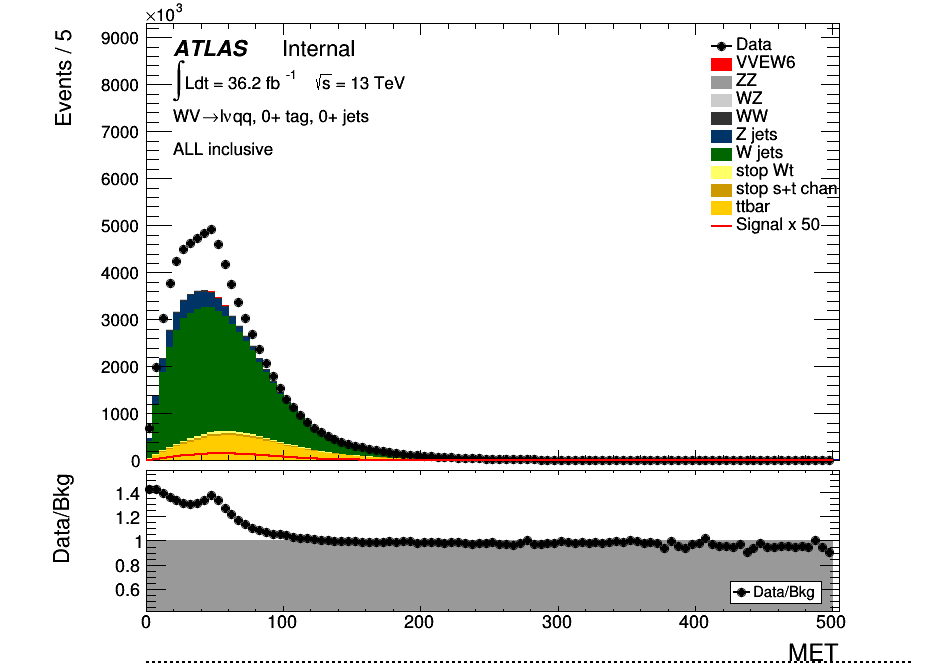
\includegraphics[width=\linewidth]{figures/1lep/CRPlots/C_0ptag0pjet_0ptv_ALL_MET_Lin.png}
            \caption{$E_{T,miss}$ before any event selection.}
        \end{subfigure}
        \begin{subfigure}{0.3\textwidth}
            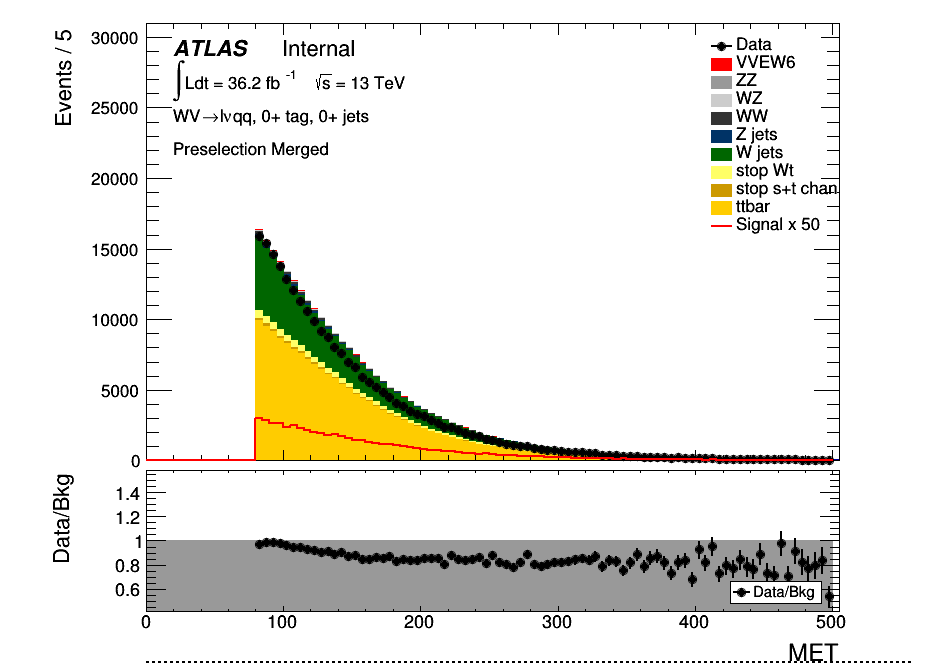
\includegraphics[width=\linewidth]{figures/1lep/CRPlots/C_0ptag0pjet_0ptv_Presel_Merged_MET_Lin.png}
            \caption{$E_{T,miss}$ after merged common preselection.}
        \end{subfigure}
        \begin{subfigure}{0.3\textwidth}
            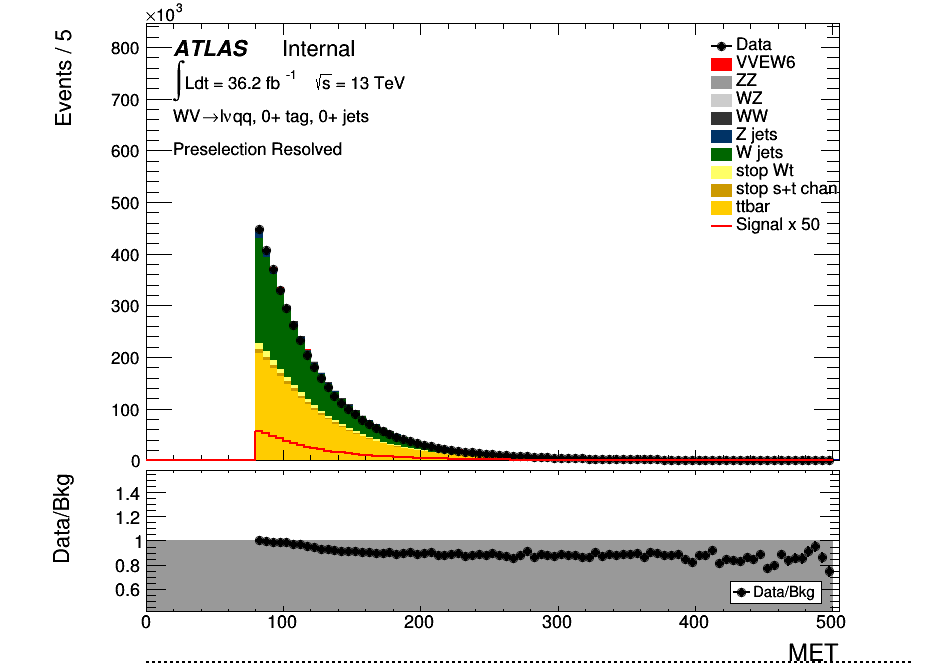
\includegraphics[width=\linewidth]{figures/1lep/CRPlots/C_0ptag0pjet_0ptv_Presel_Resolved_MET_Lin.png}
            \caption{$E_{T,miss}$ distribution after resolved common preselection.}
        \end{subfigure} \\

        \begin{subfigure}{0.3\textwidth}
            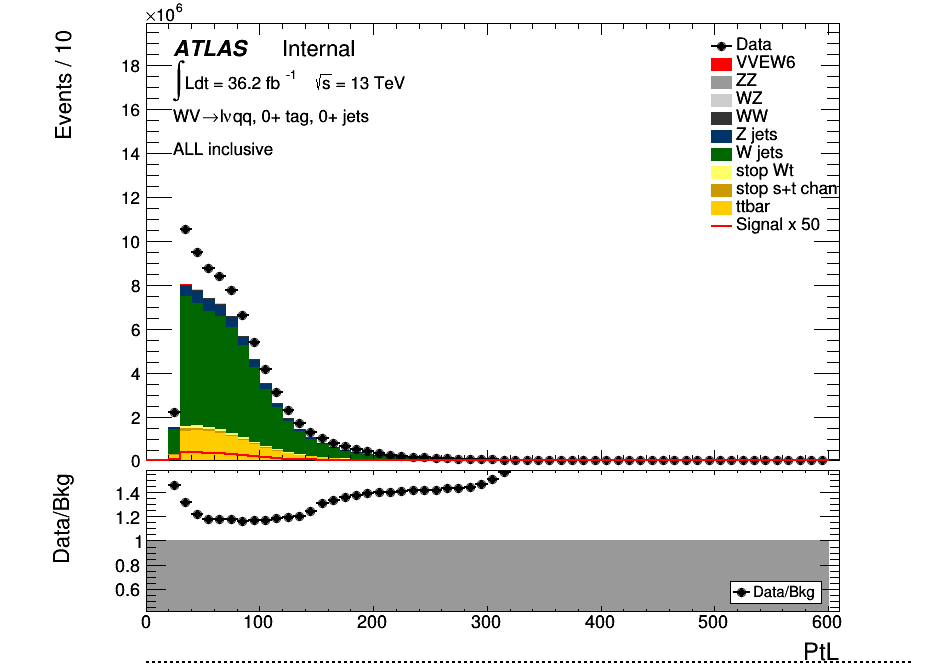
\includegraphics[width=\linewidth]{figures/1lep/CRPlots/C_0ptag0pjet_0ptv_ALL_PtL_Lin.png}
            \caption{$p_{T,l}$ before any event selection.}
        \end{subfigure}
        \begin{subfigure}{0.3\textwidth}
            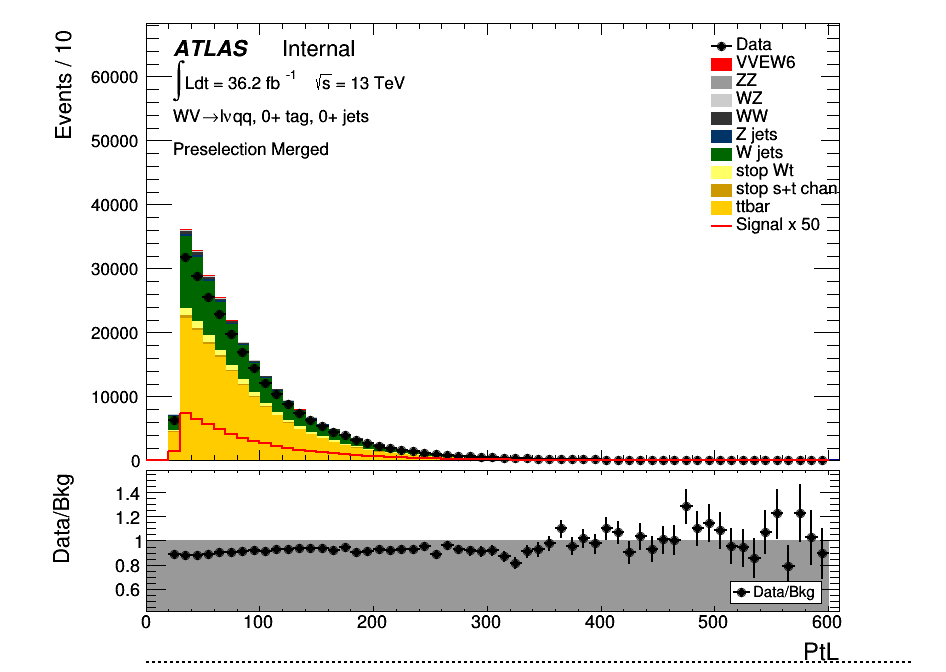
\includegraphics[width=\linewidth]{figures/1lep/CRPlots/C_0ptag0pjet_0ptv_Presel_Merged_PtL_Lin.png}
            \caption{$p_{T,l}$ after merged common preselection.}
        \end{subfigure}
        \begin{subfigure}{0.3\textwidth}
            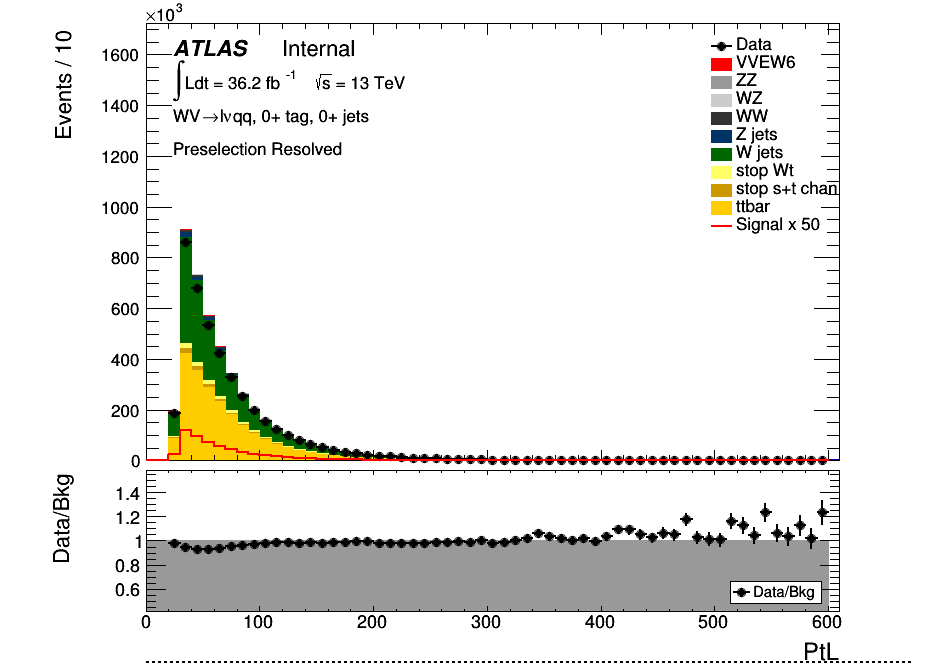
\includegraphics[width=\linewidth]{figures/1lep/CRPlots/C_0ptag0pjet_0ptv_Presel_Resolved_PtL_Lin.png}
            \caption{$p_{T,l}$ distribution after common resolved preselection.}
        \end{subfigure} \\

        \begin{subfigure}{0.3\textwidth}
            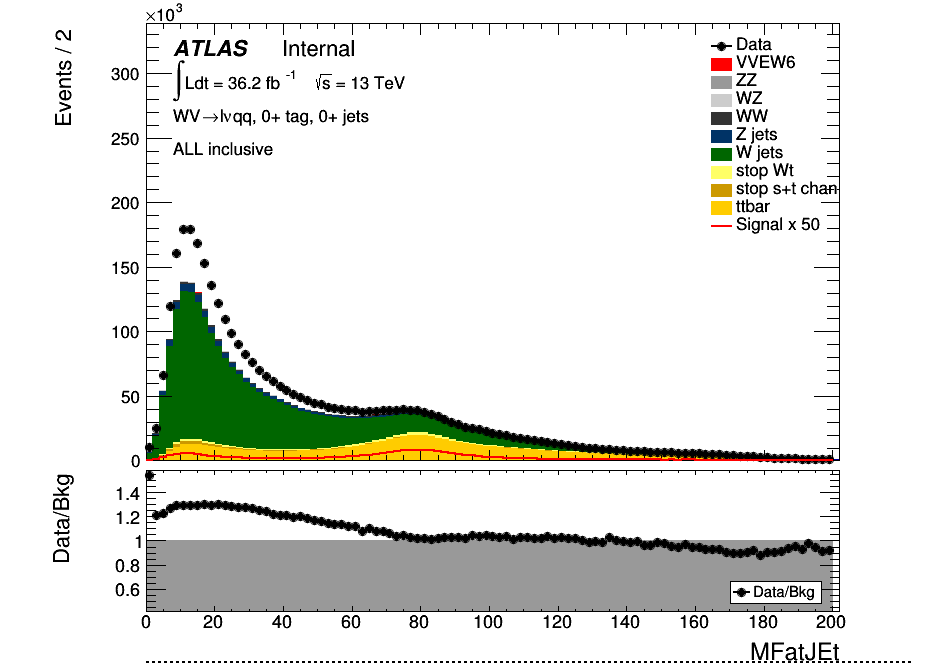
\includegraphics[width=\linewidth]{figures/1lep/CRPlots/C_0ptag0pjet_0ptv_ALL_MFatJet_Lin.png}
            \caption{$M_{J}$ before any event selection.}
        \end{subfigure}
        \begin{subfigure}{0.3\textwidth}
            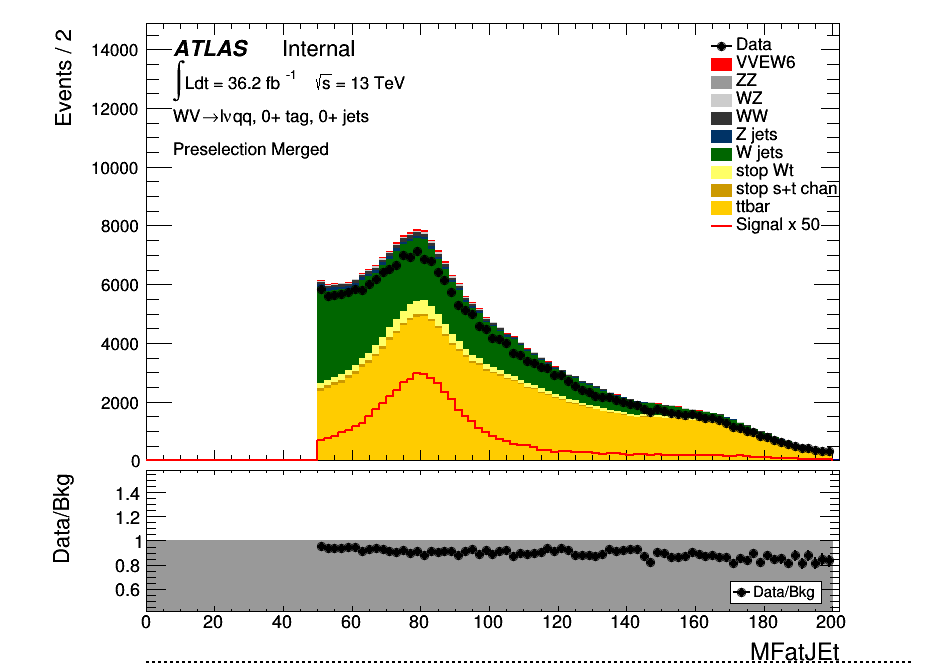
\includegraphics[width=\linewidth]{figures/1lep/CRPlots/C_0ptag0pjet_0ptv_Presel_Merged_MFatJet_Lin.png}
            \caption{$M_{J}$ after merged common preselection.}
        \end{subfigure}

        \caption{Distributions for $E_{T,miss}$, $E_{T,miss}$, and $m_{J}$ in the 1 lepton channel at different stages of the analysis selection; preselection merged and preslection resolved labels refers to the set of cuts applied in the merged and resolved regime rather than the boson tagger cuts (merged) and the signal jets mass window cut.}
        \label{fig:1LepPreselCuts}
\end{figure}


%%%\begin{figure}[ht]
%%%\centering
%%%	\subfigure[$E_{T,miss}$ before any event selection.]{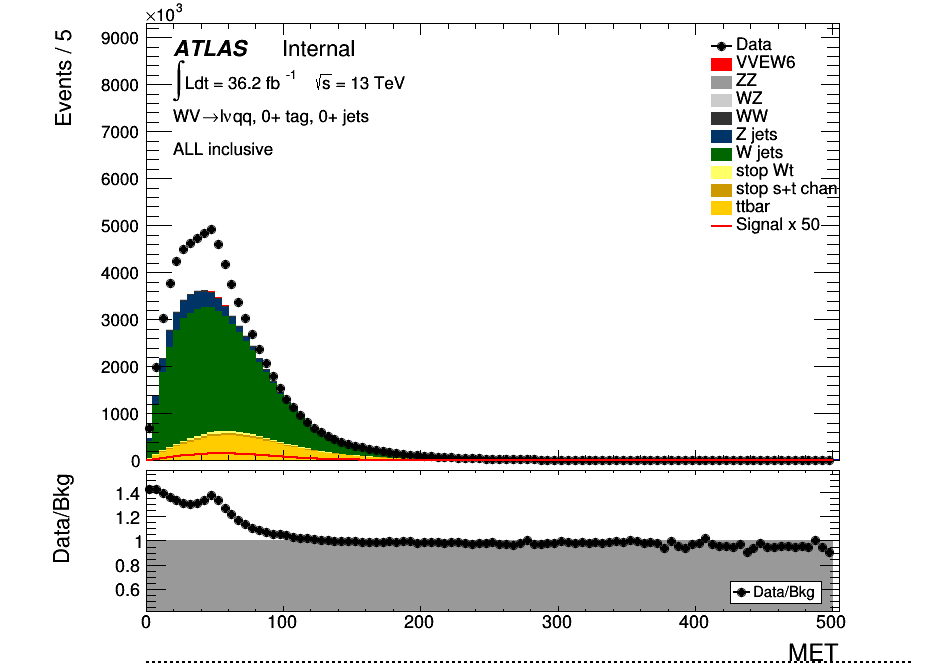
\includegraphics[width=0.3\textwidth]{figures/1lep/CRPlots/C_0ptag0pjet_0ptv_ALL_MET_Lin.png}} 
%%%	\subfigure[$E_{T,miss}$ after merged common preselection.]{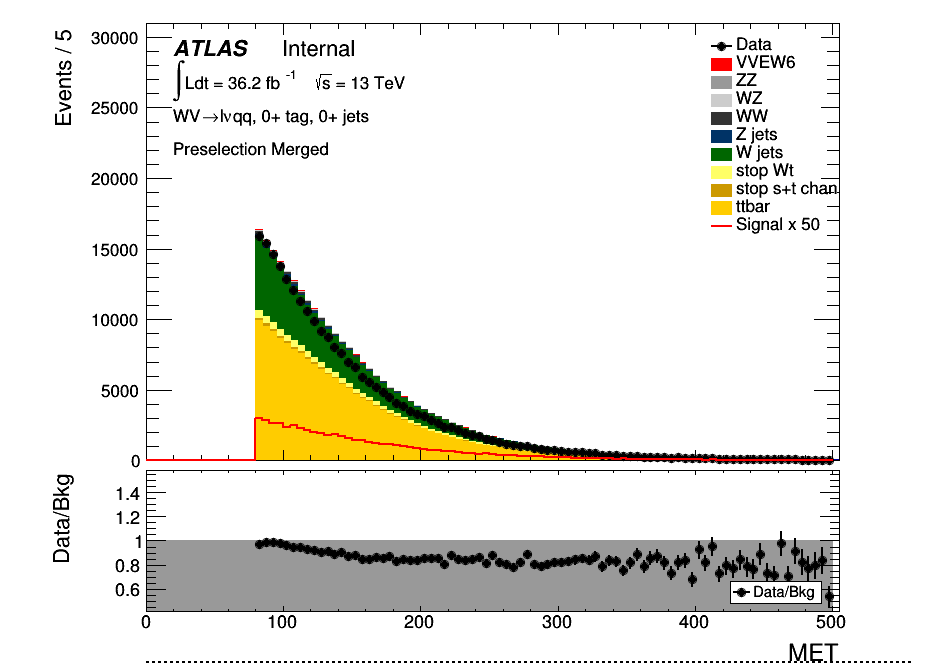
\includegraphics[width=0.3\textwidth]{figures/1lep/CRPlots/C_0ptag0pjet_0ptv_Presel_Merged_MET_Lin.png}} 
%%%	\subfigure[$E_{T,miss}$ distribution after resolved common preselection.]{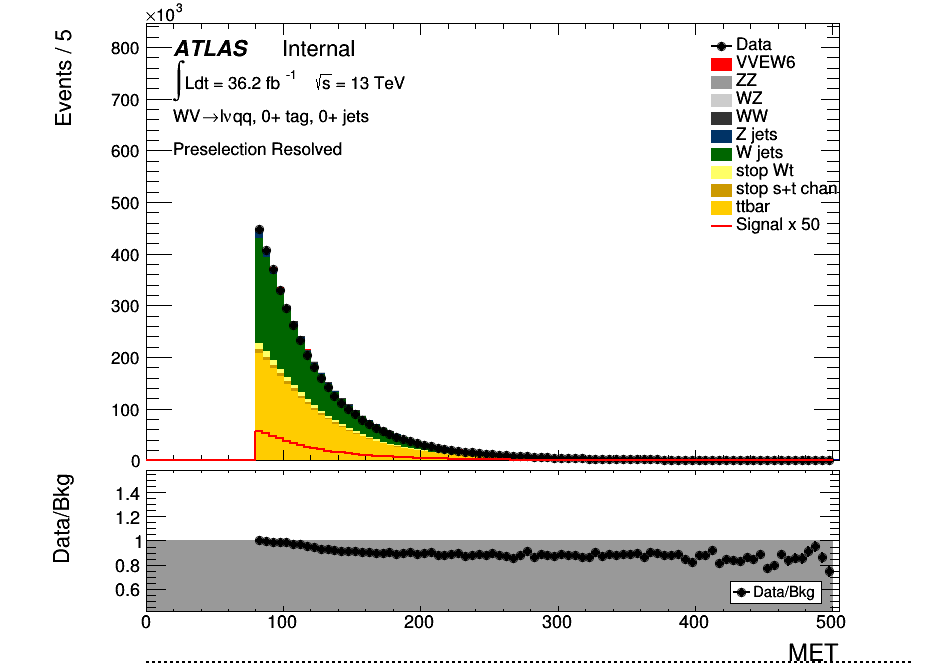
\includegraphics[width=0.3\textwidth]{figures/1lep/CRPlots/C_0ptag0pjet_0ptv_Presel_Resolved_MET_Lin.png}} \\
%%%
%%%	\subfigure[$p_{T,l}$ before any event selection.]{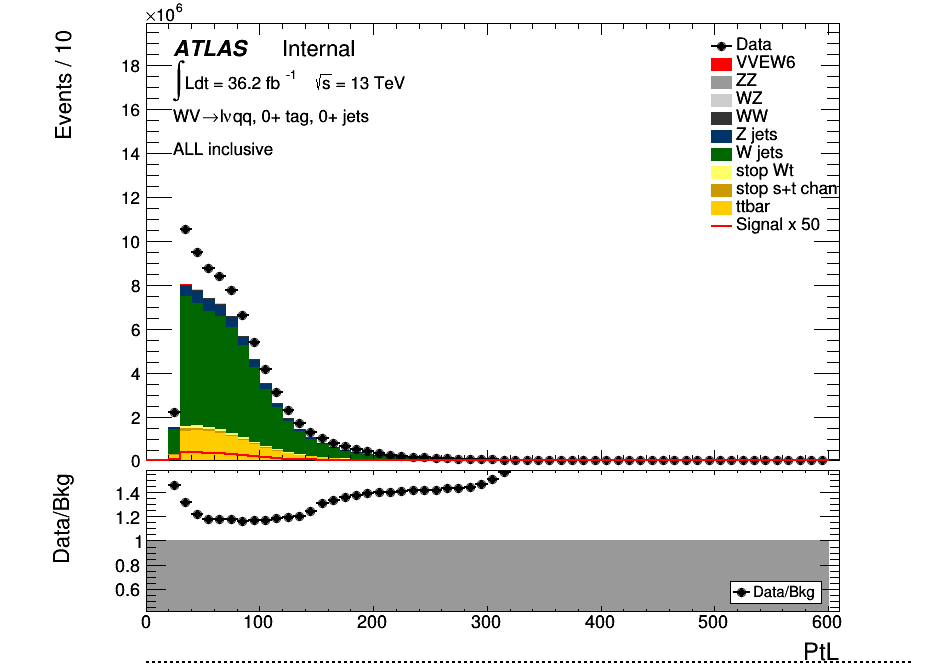
\includegraphics[width=0.3\textwidth]{figures/1lep/CRPlots/C_0ptag0pjet_0ptv_ALL_PtL_Lin.png}} 
%%%	\subfigure[$p_{T,l}$ after merged common preselection.]{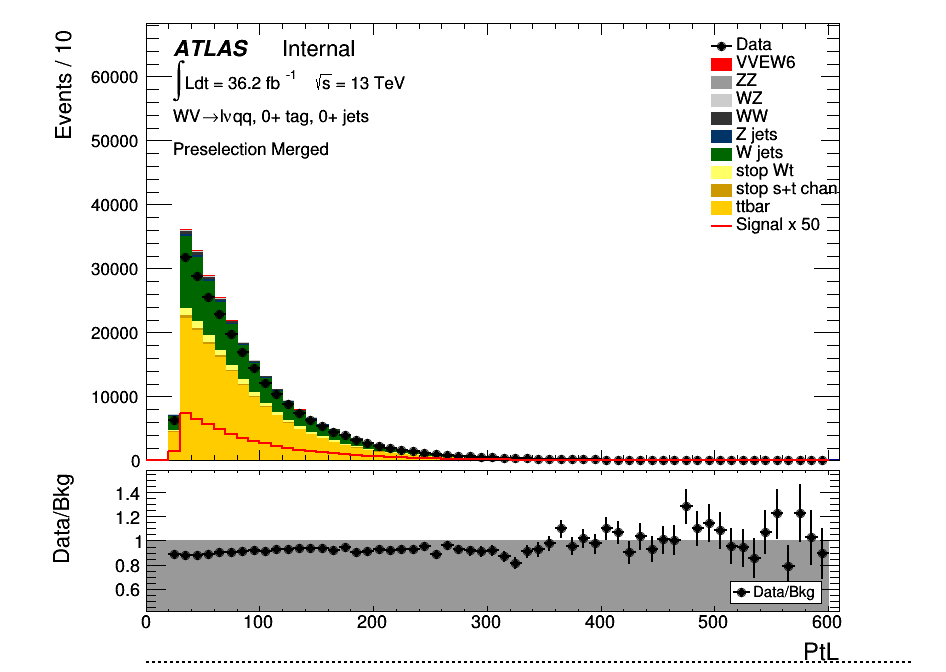
\includegraphics[width=0.3\textwidth]{figures/1lep/CRPlots/C_0ptag0pjet_0ptv_Presel_Merged_PtL_Lin.png}} 
%%%	\subfigure[$p_{T,l}$ distribution after common resolved preselection.]{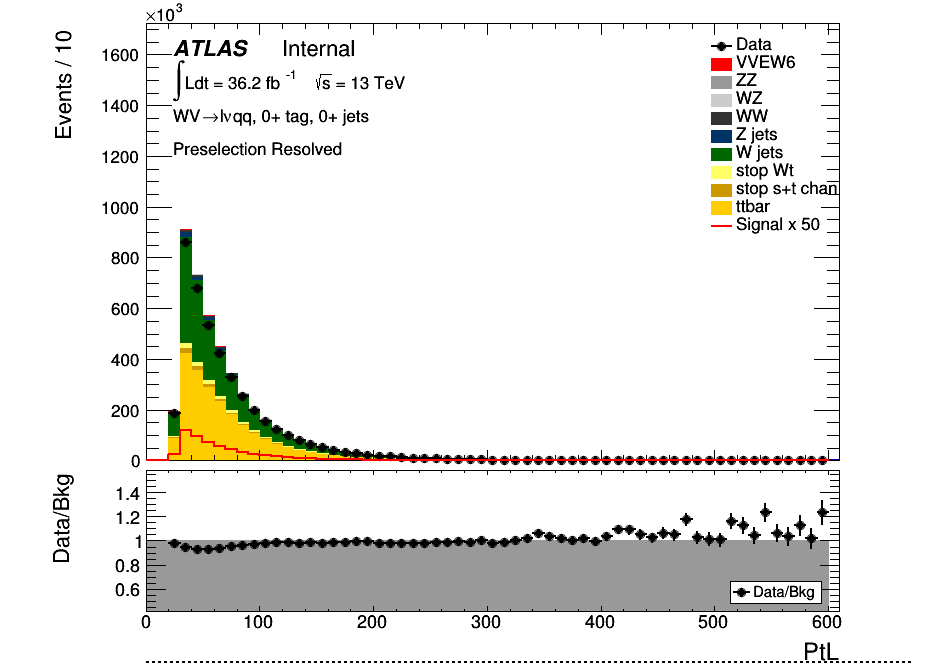
\includegraphics[width=0.3\textwidth]{figures/1lep/CRPlots/C_0ptag0pjet_0ptv_Presel_Resolved_PtL_Lin.png}} \\
%%%
%%%	\subfigure[$M_{J}$ before any event selection.]{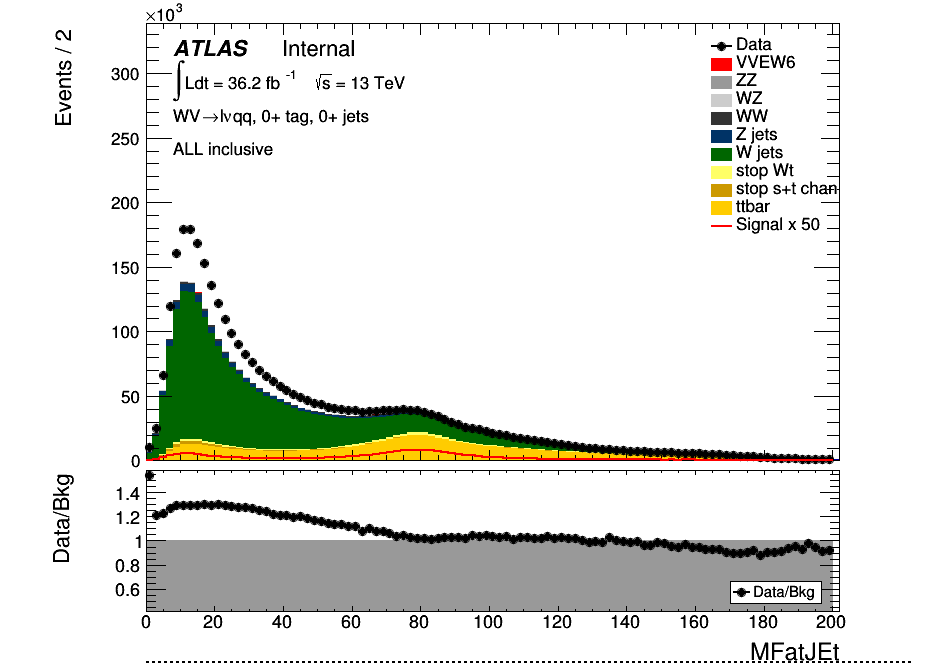
\includegraphics[width=0.3\textwidth]{figures/1lep/CRPlots/C_0ptag0pjet_0ptv_ALL_MFatJet_Lin.png}} 
%%%	\subfigure[$M_{J}$ after merged common preselection.]{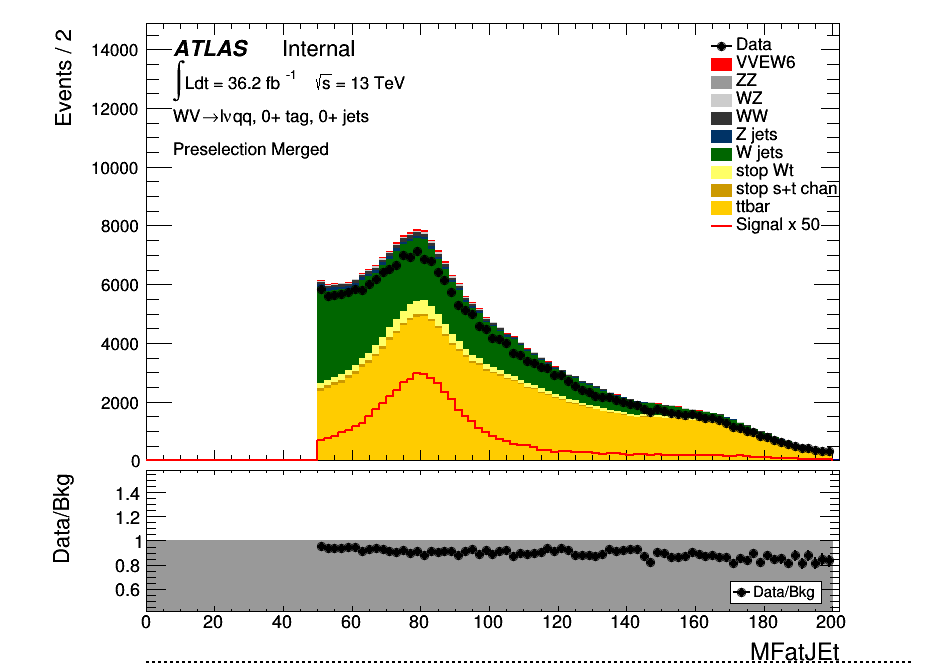
\includegraphics[width=0.3\textwidth]{figures/1lep/CRPlots/C_0ptag0pjet_0ptv_Presel_Merged_MFatJet_Lin.png}} 
%%%
%%%	\caption{Distributions for $E_{T,miss}$, $E_{T,miss}$, and $m_{J}$ in the 1 lepton channel at different stages of the analysis selection; preselection merged and preslection resolved labels refers to the set of cuts applied in the merged and resolved regime rather than the boson tagger cuts (merged) and the signal jets mass window cut.}
%%%	\label{fig:1LepPreselCuts}
%%%\end{figure}


%After the $W \to \ell\nu$ selection above and $W/Z \to jj$ selection described in Section~\ref{subsubsec:resolved_jets_selection},
%the following selection cuts are required to take the event topology of which two high-\pt\ bosons are back--to--back in the $x$--$y$ plane:
%\begin{itemize}
%\item $\Delta \phi(\ell, \met)< XX$;
%\item $\Delta \phi(j1,j2) < XX$;
%\item $\Delta \phi(\ell,j1(2)) > XX$;
%\item $\Delta \phi(j1(2), \met) > XX$;
%\end{itemize}
%where $\Delta \phi(i, j)$ is the distance in the  coordinate between objects $i$ and $j$.

%%% 2-leptons channel

%In particular, modelling of the leading and sub-leading muon \pt look slighlty different. 
%This is an effect of the first bin in both distributions that has different values in the 
%data/MC ratio. After removing the first bin in the subleading muon \pt distribution the modelling
%qfor the two muons \pt is consistent as checked in Appendix \ref{app:leptonin2lep}.


%%%
\clearpage
\section{VBS Selection}
\clearpage
\subsection{VBS Selection}
\label{subsec:vbs_selection}

In all three channels events are required to contain a small-R jet pair as a candidate VBS jets, we refer to them as Tag Jets. 

The hadronically-decaying $W/Z$ candidate is reconstructed as either two small-$R$ jets~($j$)
or one large-$R$ jet~($J$), as explained in the following sections \ref{subsubsec:merged_jets_selection}-\ref{subsubsec:resolved_jets_selection}; therefore, each event should contain at least four small-$R$ jets in the resolved analysis or one large-$R$ jet and
two small-$R$ jets in the merged analysis. 

The strategy to select first tag jets and then signal jets which came from $W/Z$ from the remaining jets is chosen; 
this is motivated from the preference to focus on the production topology first (VBS jets) 
and then move to identify the objects related to the decay part of the target process. 
%Furthermore, this choice is consistent what the strategy performed in the VV semi-leptonic resonant search \cite{Bachas:2646593}.

The tagging jets algorithm is quite usual to what is done in analyses in ATLAS.

Tagging jets are required, 
firstly, 
%to be non-$b$-tagged; this would help in order to suppress the contribution of diagrams with a $Wtb$ vertex
%(especially the electroweak $t\bar{t}$ production) in the electroweak $VVjj$ production. 
%Furthermore, 
%fJVT selection has been applied to the small-R jets; 
to pass the fJVT selection, the Loose fJVT WP is used.
%the jets are required to pass the Loose fJVT WP as additional criteria to be selected as tagging jets. 
The Loose WP has been chosen for simplicity, indeed, it is the default WP recommended 
and the related SF are by default available in our analysis framework; 
furthermore, no significant difference with respect to the Tight WP has been observed, 
more details are given in dedicated studies reported in appendix \ref{app:fjvt}.
Furthermore, b-veto has been investigated to be applied on all the jets of the collection
before pairing the candidates, since, no significant impacts has been found,
as documented in the Appendix \ref{app:tagjet_bveto}, no b-jet requirement is applied on the taggging jets.

The tagging jets candidates must be in the opposite hemispheres, 
$\eta_{\mathrm{tag}\ j_1} \cdot \eta_{\mathrm{tag}\ j_2} < 0$,
and to have the highest dijet invariant mass among all the possible pairs of small-R jets in the event, 
that have passed already 
%b-tagging veto and 
the fJVT requirement, as mentioned above.
 
After the tagging jet pair are selected, it is required that both tagging jets should have \pT$>$30~\GeV and that the invariant mass of the two tagging jets system is greater than 400~\GeV; 
%we rely on the optimisation studies done in the previous round of the analysis on the choice of both \pT and invariant mass cuts. 
As an example, the \mjjtag distribution for both data and MC samples is shown before the cut in the \zlep channel SRs Figure \ref{fig:0lepMjj}; 
the \mjjtag re-weighting is already applied and it will be described in section \ref{subsec:mjj_reweight}.

\begin{figure}[ht]
    \centering
    \subfigure[merged HighPurity]{\includegraphics[width=0.3\textwidth]{figures/0lep/cutflow/nominal/merged/plots/soverb_individual_SRVBS_HP_MTagMerJets400_MTagMerJets_cutflow.pdf}}
    \subfigure[merged LowPurity]{\includegraphics[width=0.3\textwidth]{figures/0lep/cutflow/nominal/merged/plots/soverb_individual_SRVBS_LP_MTagMerJets400_MTagMerJets_cutflow.pdf}}
    \subfigure[resolved]{\includegraphics[width=0.3\textwidth]{figures/0lep/cutflow/nominal/merged/plots/soverb_individual_SRVBS_Res_MTagResJets400_MTagResJets_cutflow.pdf}}
    \caption{0-lepton $m(jj)^\text{tag}$ selection. The distributions are shown for the three SR selections; the specific definition of each of them (HighPurity, LowPurity, Resolved) will be given in the following Section \ref{subsec:sr_selection}. Entering are events passing the respective selection up to the point of the $m(jj)^\text{tag}$ cut which is shown by the vertical line.} 
    \label{fig:0lepMjj}
\end{figure}




%%%
\clearpage
\section{Signal Regions (SRs) Selection}
%%\clearpage
%%\subsection{Signal Regions (SRs) definitions}
\label{subsec:sr_selection}

Multiple Signal Regions (SRs) are defined to optimize the signal sensitivity and to accommodate the different reconstruction regimes of the hadronically decaying boson ($V \rightarrow qq$). The Merged regime is prioritized over the Resolved regime. Detailed descriptions of these two regimes are provided in this section.

%\subsection{Selection of $W/Z \to J$ candidates (merged category)}
\subsection{Selection of \texorpdfstring{$W/Z \to J$}{W/Z -> J} candidates (merged category)}
\label{subsubsec:merged_jets_selection}

For boosted (high-energy) boson production, where the \pt of hadronically decaying $W/Z$ bosons is at least 200 GeV, each boson is frequently reconstructed as a single large-$R$ jet. In this ``merged'' category, the selection requires at least one large-$R$ jet, with the leading large-$R$ jet utilized for $W/Z$ candidate reconstruction. To avoid double-counting jet energy, the large-$R$ jet must be separated by a distance greater than $|\Delta R| = 1.4$ from both VBS Tag Jets.
%
The final step in selecting boosted $W/Z \to qq$ candidates involves boson tagging based on three variables: jet mass ($m_{J}$), substructure variable $D_2$, and ungroomed track multiplicity ($n_{\text{Tracks}}$).
We adopt tagger working points (WPs) recommended for $50\%$ and $80\%$ signal efficiencies, applied at the jet level to optimize the selection.

To establish orthogonal regions, we define:
\begin{itemize}
    \item High-Purity (HP) Region: Includes events (and their corresponding single large-R jet) that meet the $50\%$ WP criteria.
    \item Low-Purity (LP) Region: Includes events that satisfy the $80\%$ WP but do not fulfill the $50\%$ WP criteria.
\end{itemize}
Thus, events in the merged regime conforming to the $50\%$ WP criteria are categorized into the HP Signal Region (SR), while those meeting the $80\%$ WP standards but not the $50\%$ are allocated to the LP SR. Table~\ref{tab:1lep_merged} contains the complete definitions of the HP and LP SRs.

For the HP SR, the $50\%$ WP $W/Z$-tagging scale factor is applied. For the LP SR, a custom scale factor is defined:

    \begin{equation}
    SF_{LP} = \frac{\epsilon_{loose}SF_{eff,loose}- \epsilon_{tight}SF_{eff,tight} }{ \epsilon_{loose}- \epsilon_{tight}}
    \end{equation}
Here, $\epsilon$ represents the efficiency estimated in \ttbar events for signal and $\gamma$+jets and multijet events for background.
``Loose'' corresponds to the $80\%$ WP, while ``tight'' refers to the $50\%$ WP. Detailed discussions on $W/Z$-tagging scale factors are available in Section \ref{subsec:bkg_uncer_vtagger}.

In the baseline boson tagger, exclusive selections for $Z$ and $W$ candidates are used. However, due to significant overlap in these selections, it is not feasible to define two orthogonal regions for the hadronic decays of $W$ and $Z$. Therefore, an inclusive $V \to qq$ selection is utilized, which is a logical OR of the $W$ and $Z$ boson tagger selections. This inclusive selection adopts the lower mass cut from the $W$ selection and the upper cut from the $Z$ selection.


\subsection{Selection of $W/Z \to jj$ candidates (resolved category)}
\label{subsubsec:resolved_jets_selection}

In the lower \pt range for hadronically decaying $W/Z$ bosons, two distinct jets are typically resolvable. This resolved regime offers the highest efficiency for EW $VV+jj$ signals, although its sensitivity is marginally lower compared to the merged regime due to increased background acceptance.
Within this regime, events are selected based on the presence of at least two ``signal'' jets. These signal jets are identified from a pool of candidates, excluding the two VBS Tag Jets.

In the search of $W/Z$ candidates, we select the two signal jets with the highest \pt. This approach slightly reduces signal efficiency within the mass window compared to previous analyses. However, it allows for a more relaxed application of the Close-$V$ selection algorithm, which pairs jets with invariant masses closest to the nominal $V$($W/Z$) boson masses. 

After selecting the two jets of interest, the leading jet is required to have \pt $\SI{>40}{\GeV}$, a criterion set to further reduce background and enhance sensitivity. To identify events indicative of a hadronically decaying $W/Z$ boson, the dijet mass ($m_{jj}$) is constrained within a mass window of $64 <m_{jj}<106\,\GeV$.

Figure~\ref{fig:1lepMVHadResSR} shows the full range distributions for $m_{jj}$ without the mass window constraints, with the $W$ peak coming from top-associated processes clearly visible.

As mentioned in Section~\ref{sec:mc_sample_ewvvjj}, a VBS-enhancing cut, $m_{jjj} > 220\,\si{\GeV}$, is introduced later in the analysis to reduce the contribution from the non-VBS $tZb$ process, as illustrated in Fig.~\ref{fig:feynmantZb}. This cut, implemented near the reconstructed top mass, is shown in Figure~\ref{fig:1lepWCR_mjjj} in the next section. Events passing this cut are classified into ``tight'' regions, while those that do not are classified into ``loose'' regions. The resolved ``tight'' regions are used in calculations and statistical studies, whereas the resolved ``loose'' regions serve as a sanity check.

\begin{figure}[ht]
    \centering
    \begin{subfigure}{0.32\textwidth}
        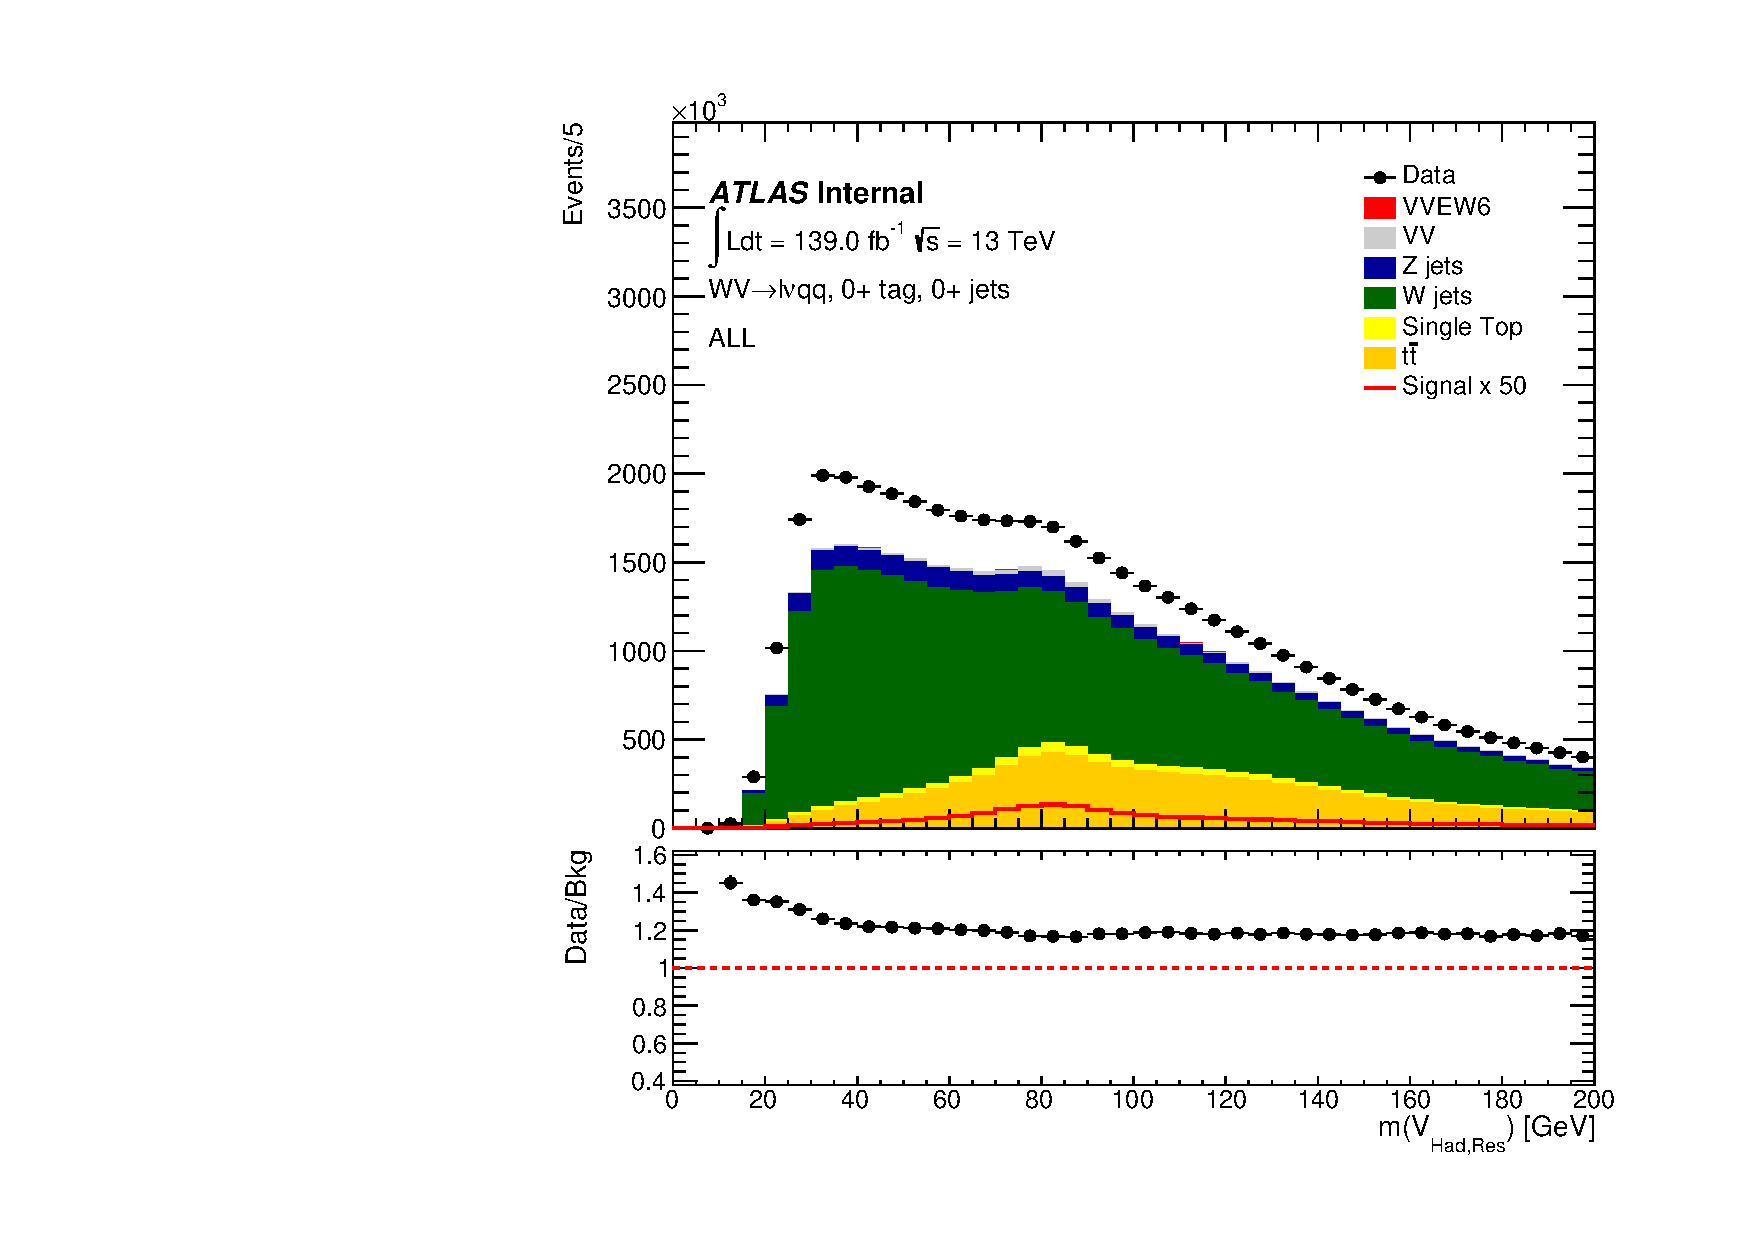
\includegraphics[width=\linewidth]{figures/event_selection/ALL_MVHadRes.pdf}
        \caption{Before any event selection.}
    \end{subfigure}
    \begin{subfigure}{0.32\textwidth}
        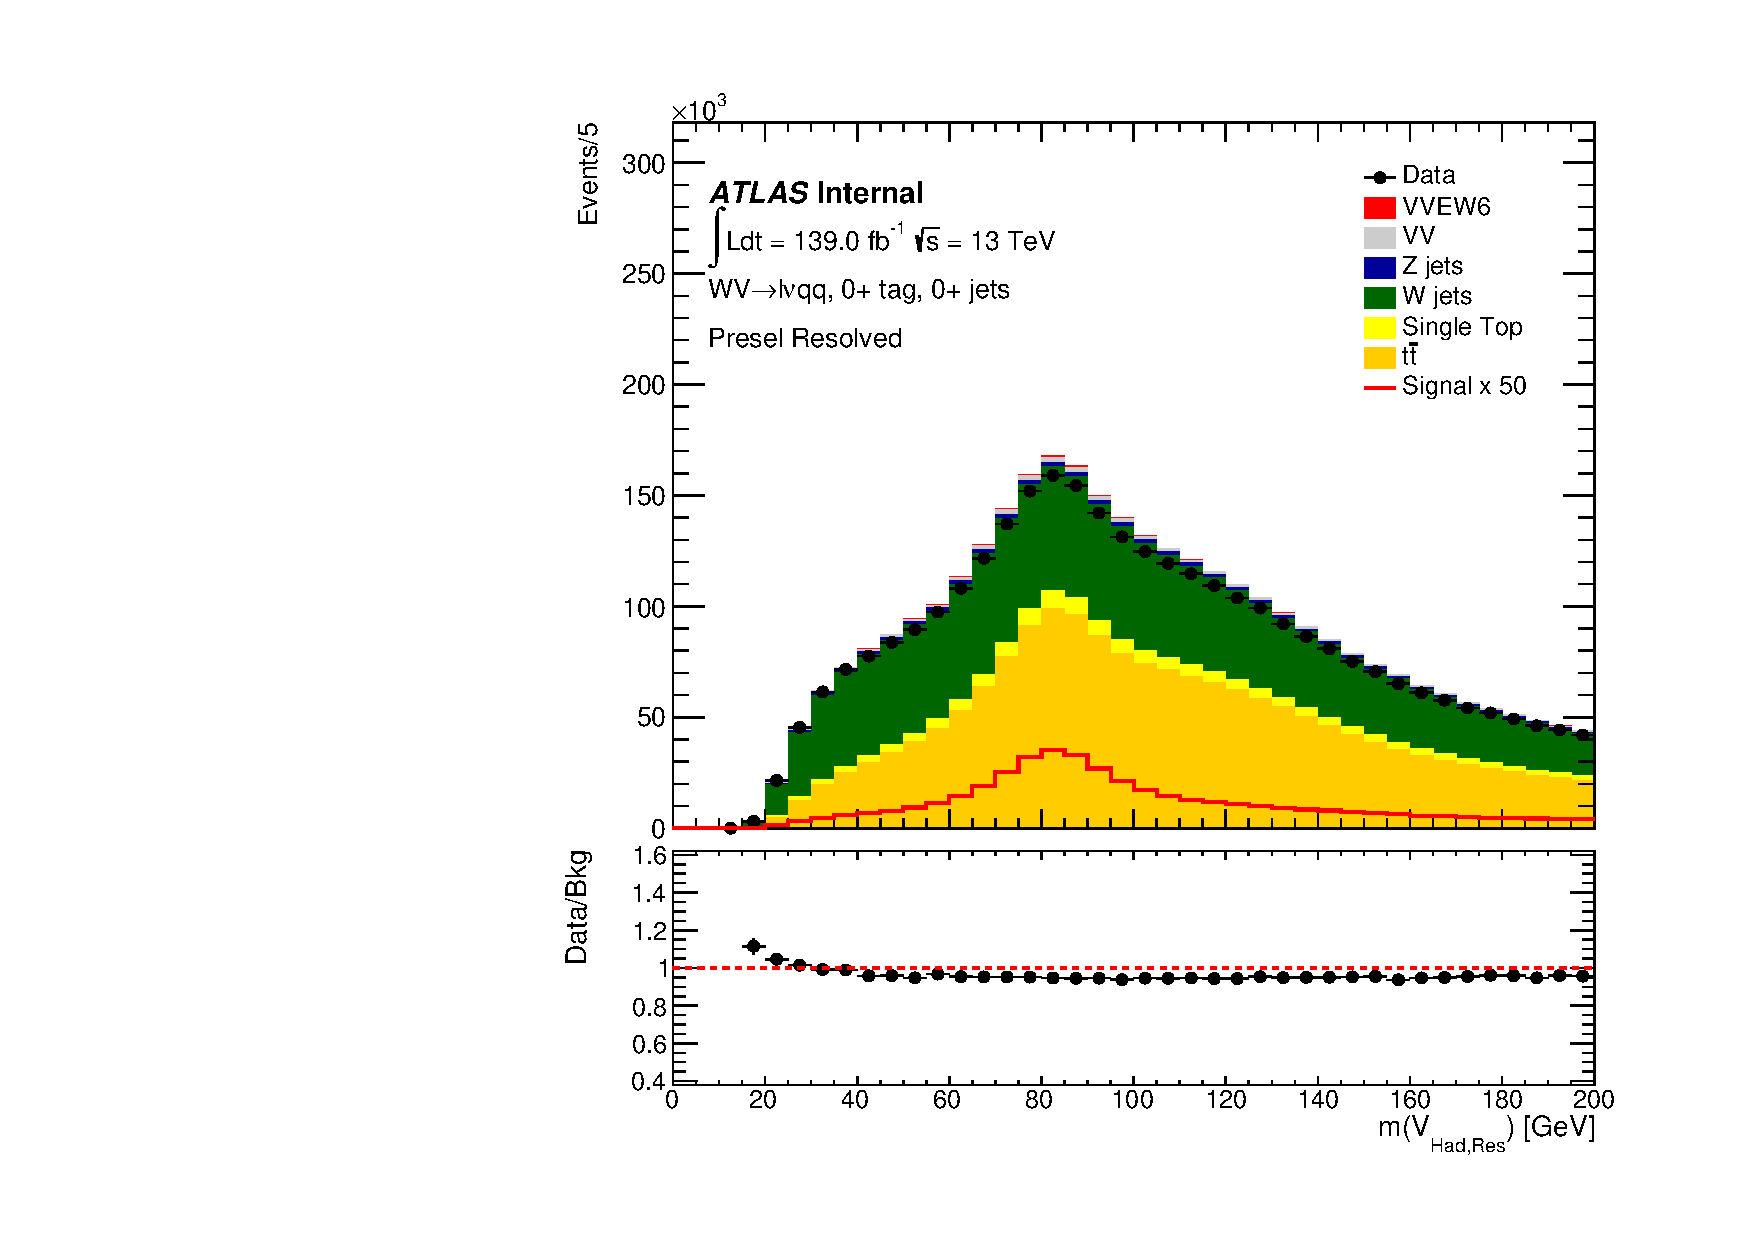
\includegraphics[width=\linewidth]{figures/event_selection/Presel_Resolved_MVHadRes.pdf}
        \caption{After resolved preselection.}
    \end{subfigure}
    \caption{Reconstructed mass distribution of the leading two jets.}
    \label{fig:1lepMVHadResSR}
\end{figure}

\subsection{VV system invariant mass}
\label{subsubsec:mVV_reconstruction}

The mass of the $WV$ system, $m_{WV}$, is calculated using the lepton, neutrino, and the hadronically-decaying boson (represented by either a large-$R$ jet or two small-$R$ jets). To determine the neutrino's momentum in the $z$-direction ($p_z$), we apply the Particle Data Group (PDG) value for the $W$ boson mass to the lepton-neutrino system. This results in a quadratic equation. The solution for $p_z$ is chosen based on the following criteria: if the solutions are complex, the real component is taken; if they are real, the solution with the smaller absolute value is selected.

%%%%%

%%%
%%%\subsection{EW Top production veto}
\subsubsection{EW Top production veto: Tight region definition}
\label{subsec:topveto_selection}

We found that the contribution of the EW Top production is still significant in our SRs. 

As discussed in Section~\ref{sec:mc_sample_ewvvjj},
the EW Top and VVV processes are included in the signal MC samples. Since we want to enhance the VBS processes in our target phase space for the interpretation of data/MC agreement with the aQGC new physics model, we add additional selections to reduce the top contribution.

%\textcolor{red}{put here a table of the VV, VVV and top contributions in the SRs}

%\subsubsection{Loose and tight regions definition}
\label{subsec:LooseTightRegion}

We found that the resolved regions have much higher top contribution with respect to the merged ones.
For the top contribution in our signal sample, the top-quark mass can be reconstructed in the resolved SRs.
Two signal jets and the additional third jet which forms the three-jet mass, $m_{jjj}$, 
the closest to the top mass (172.76 \ GeV) are used. 
Additional third jet was chosen from all jets except for signal jets, including VBS tagging jets.
Figure \ref{fig:2leptopMass}-a shows the $m_{jjj}$ distributions for top contribution, VVV, and other components (e.g. VBS) in the EW WZjj signal sample.
We can reject the top contribution by the cut on $M_{jjj}$ at 220~\GeV.
Figure \ref{fig:2leptopMass}-b shows the data/MC comparison of the $M_{jjj}$ distribution in the \tlep \Zjets CR.
The mis-modelling in Z+jets shown in $m_{tagjj}$ was also seen in $M_{jjj}$ distribution. It is also corrected by re-weighting with $m_{tagjj}$ described in section~\ref{subsec:mjj_reweight}, though a slight slope is seen in figure \ref{fig:2leptopMass}-b, which seems to be re-weighted a little too much in this phase space.

\begin{figure}[ht]
    \begin{center}
    	\subfigure[$\text{top mass peak}$]{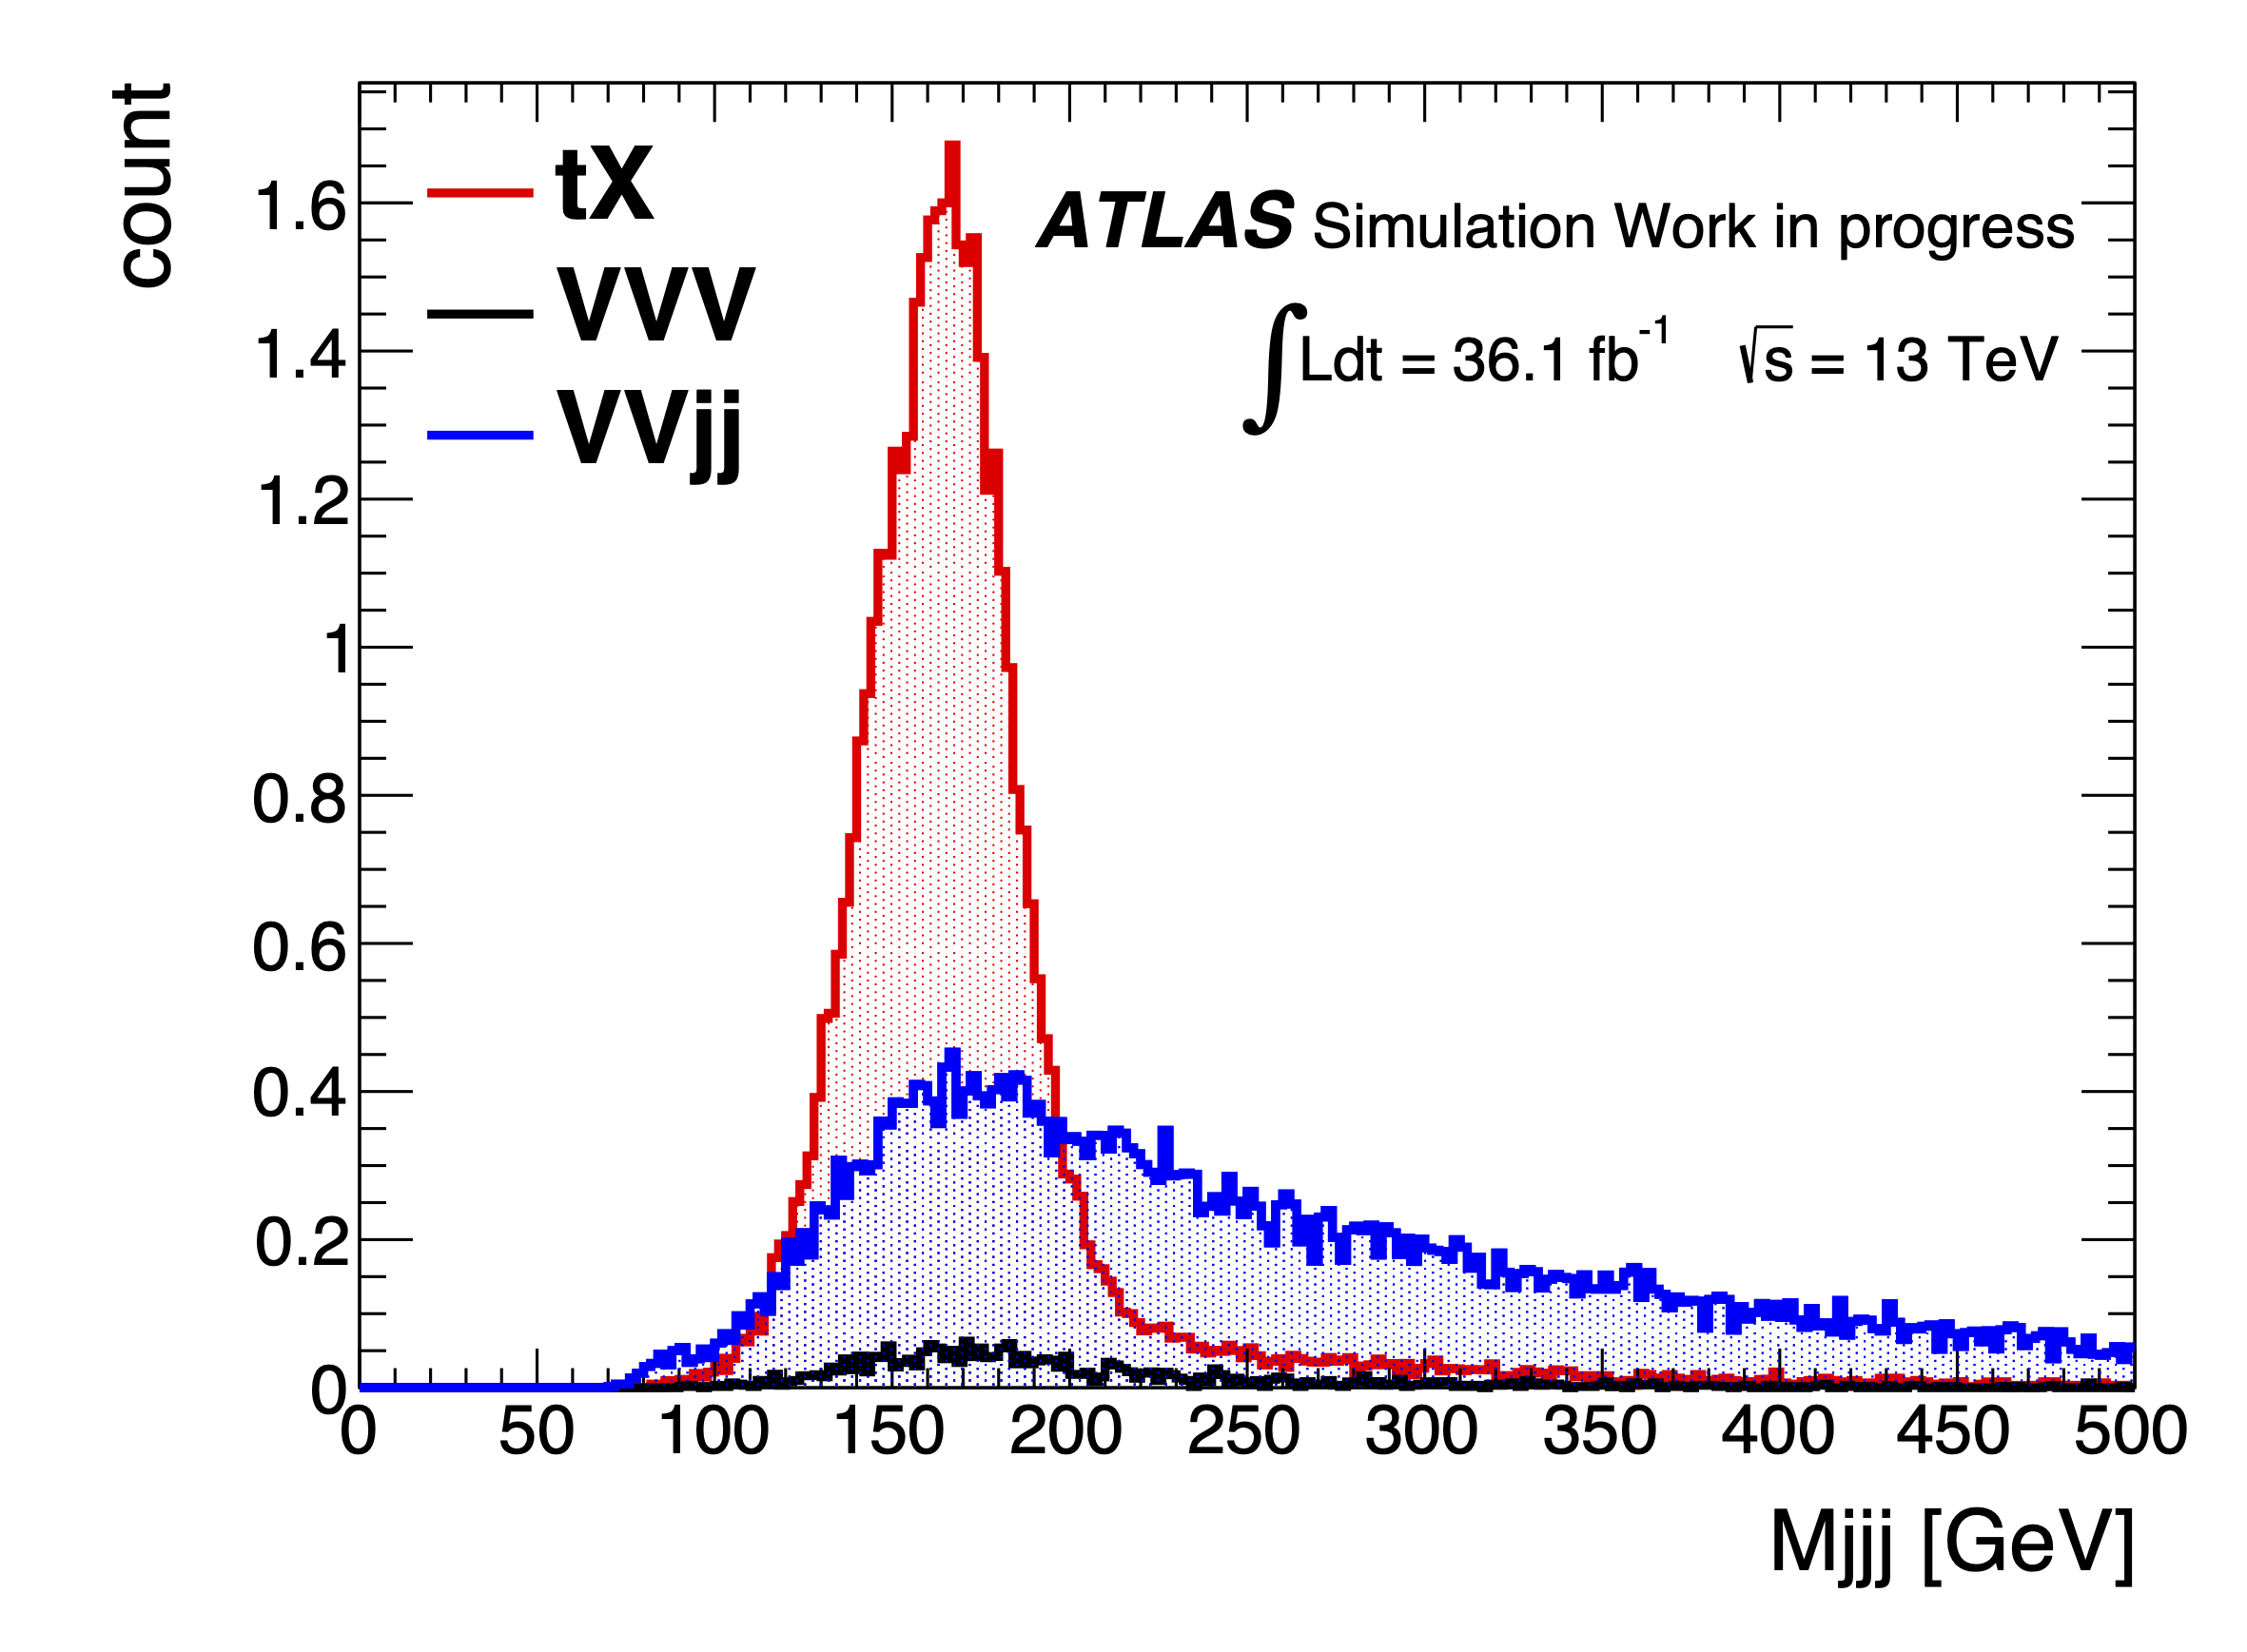
\includegraphics[width=0.4\textwidth]{figures/2lep/topMass/WZjjtopMasspeak.png}}
    	\subfigure[$\text{top mass in CRVjet}$]{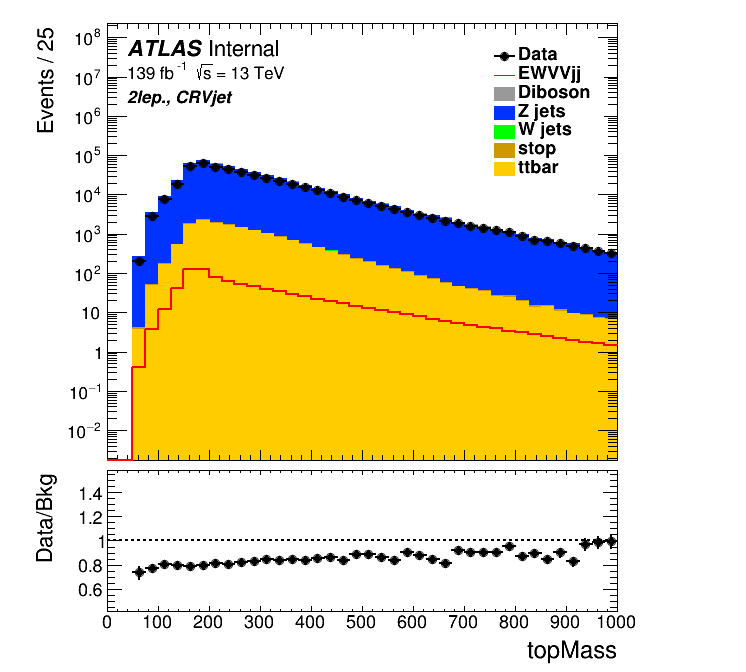
\includegraphics[width=0.4\textwidth]{figures/2lep/dataMC/C_0ptag2pjet_0ptv_CRVjet_topMass_Log.png}}
        \caption{ Mass of 3 jets in the 2-lepton channel; shapes of the signal components in the Resolved SR (a) and data to MC comparison in the \Zjets CR (b) are shown.} 
        \label{fig:2leptopMass}
    \end{center}
\end{figure}

Figure \ref{fig:0leptopMass} shows distributions for the reconstructed top mass in the \zlep channel; 
in particular, only data, signal and top background are shown to stress the most of the top background 
is rejected by this cut, while the actual data, containing the other SM background as well as the EWK signal
have higher selection efficiency in the high reconstructed top mass. 
Furthermore, the bottom pannel shows the signal to background ration that in increasing with this variable.

\begin{figure}[ht]
    \begin{center}
    	\subfigure[merged HP SR]{\includegraphics[width=0.45\textwidth]{figures/0lep/cutflow/topcheck/merged/plots/soverb_individual_SRVBS_HP_cutTopMassMer_topMassMer_cutflow.pdf}}
    	\subfigure[resolved SR]{\includegraphics[width=0.45\textwidth]{figures/0lep/cutflow/topcheck/merged/plots/soverb_individual_SRVBS_Res_cutTopMassRes_topMassRes_cutflow.pdf}}
        \caption{ Mass of $J^\text{sig}j^\text{extra}$ in merged (left) and of 3 jets $(jj)^\text{sig}j^\text{extra}$ in resolved in the \zlep channel signal regions. In particular, only the top background is shown, actual data contains also the other SM background, therefore, the data/MC is not expected to overlaid in the top pannel.} 
        \label{fig:0leptopMass}
    \end{center}
\end{figure}

The resolved SRs are divided into two sub-categories:
\begin{itemize}
  \item Loose Resolved: this is the baseline region defined in Section~\ref{subsubsec:resolved_jets_selection}, and
  \item Tight Resolved: Loose Resolved + $M_{jjj} > 220 GeV$.
\end{itemize}

\subsubsection{Signal purity in merged and resolved regimes}
\label{subsec:SignalPurity}

The contribution of the three truth components of the EW signal has been checked with previous SR definition and with new $M_{jjj}$ selections. 

Tables
\ref{tab:0leptopMassTable}-
\ref{tab:TruthTop1LepPurity}-
\ref{tab:TruthTop2LepPurity}
%shows the summary for the \olep channel; 
show the summary of purity picture applying the tight cut for the resolved and merged regimes 
respectively, in the \zlep-\olep-\tlep channels.

Based on the improvements and studies performed, the reconstructed top-mass cut is only applied in the resolved signal region to define the new tight signal region, and the merged signal regions are left as they are.

\begin{table}[ht]
    \centering
    \begin{tabular}{r|c|c|c|c}
         & \multicolumn{2}{c|}{merged HP SR} & \multicolumn{2}{c}{resolved SR}\\
         & before cut & after cut & before cut & after cut\\
         \hline
         truth top fraction in signal MC & $17\%$ & $13\%$ &$33\%$ & $9\%$ \\
         signal MC events & $94$ & $77$ & $594$ & $219$ \\
         top ($t\bar t$ + single $t$) MC events & $1786$ & $819$ & $18208$ & $1642$ \\
        \end{tabular}
        \caption{Effect of 3 jet cut in 0-lepton merged HP and resolved SR.} 
        \label{tab:0leptopMassTable}
\end{table}

\begin{table}[ht]
    \centering
	\resizebox{0.7\textwidth}{!}{
	\begin{tabular}{|c||c|c||c |c|}
    \hline
        & \shortstack{ VBS enhanced \\(resolved)} & \shortstack{non VBS enhanced \\ (resolved)} & \shortstack{VBS enhanced \\ (merged)} & \shortstack{non VBS enhanced \\ (merged)}\\
    \hline
    Truth Top       & 56.3 & 135.7 & 6.42 & 8.05 \\ 
    \hline
    Truth Triboson  & 3.85 & 9.08 & 1.72 &  2.178\\
    \hline
    Truth VBS       &  148 & 224.9 & 43.8 & 47.58\\
    \hline
    VBS purity & .711 & .608 & .843 & .823 \\
    \hline
	\end{tabular}}
    \caption{Event yields for 1lepton EW6 events in the resolved signal region and high purity merged signal region. The resolved VBS enhanced signal region is defined as events that pass the loose resolved signal region and pass $M_{jjj} >$ 220GeV. The merged VBS enhanced region is defined as events that pass the usual merged high purity signal region and pass $M_{Jj} >$ 220Gev, where $M_{Jj}$ is defined similarly to $M_{jjj}$, as the mass of the large-R jet and a third jet with total mass closest to the top mass. non-VBS enhanced regions are the old loose signal region definitions. 
%Based on the improvements shown here, the $M_{jjj}$ cut is only applied in the resolved signal region to define the new tight signal region, and the merged signal regions are left as they are. 
    }
\label{tab:TruthTop1LepPurity}
\end{table}

\begin{table}[ht]
    \centering
	\resizebox{0.70\textwidth}{!}{
	\begin{tabular}{|c||c|c|c|c|}      
        \hline
                    & SRVBS (resolved) & VBS enhanced (resolved) & SRVBS (merged) & VBS enhanced (merged) \\ \hline
    Truth Top       & 0.48             & 0.14                    & 0.14           & 0.10                  \\ \hline
    Truth VVV       & 0.03             & 0.03                    & 0.08           & 0.08                  \\ \hline
    Truth VBS       & 0.49             & 0.83                    & 0.78           & 0.82                  \\ \hline
	\end{tabular}
    }
    \caption{Fraction of event yields for 2lepton channel. Only EWWZjj events are checked here since there are no Top contributions in EWZZjj events.}
    \label{tab:TruthTop2LepPurity}
\end{table}

%\textcolor{red}{we put here the purities of the MC signal samples in the final reco regions comparing the diagram based classification for VV, VVV and EWTop}

%%%
\clearpage
\section{Control Regions (CRs) Definitions}
\clearpage
\subsection{Control Regions (CRs) definitions}
\label{subsec:cr_selection}

We use a combined MC template and data-driven background estimation, indeed, we rely on the MC simulations samples for the SM background processes, but we use dedicated Control Regions (CRs) to constrain the normalization of the background expectation in the SRs.

The dedicated CRs to the $Z$+jets, $W$+jets and \ttbar events are defined in this section.

The $Z$+jets, $W$+jets and \ttbar CRs are used in this analysis shared 
across the the 0-, 1- and 2-lepton channels;
for instance, the \ttbar CR is defined using \olep events only, 
and used to constraint this background in all the SRs.
Independent CRs for resolved and merged categories are, instead,
used to account for possible mis-modelling of the background depending on \pt range.

\subsubsection{$W$+jets CR (WCR) and $Z$+jets CR (ZCR)}
%\textbf{$W$+jets CR (WCR) and $Z$+jets CR (ZCR)}

The $V$+jets CR (VCR) for $V=W/Z$, $W$+jets CR (WCR), and $Z$+jets CR (ZCR) are defined using the mass sidebands with respect to hadronically decaying vector boson in 0-, 1-, and 2-lepton channels, respectively.
The event selections are otherwise the same as the SR selections.
For the simplicity of the analysis, the common sideband is defined as the outside of both $W\to q\bar{q}$ and $Z \to q\bar{q}$ signal regions.
The same definition is used in all channels:
In the resolved category, a requirement of $50 < m_{jj} < 64$ GeV or $m_{jj} > 106$ GeV is applied which is an inversion of the $m_{jj}$ cut in the corresponding SR.
In the merged case, the event has to fail the vector boson tagger's lower working point of $\epsilon=80\%$.
%In the merged category, the purity of the $W$+jets background is 77\,\% in the lower mass side band, 62\,\% in the higher mass side band region and 65\,\% in total. The $t\bar{t}$ contamination is 30\,\% in higher mass side band regions. 

Figure \ref{fig:1lep2lepMVHadResCR} shows an example of sideband distributions in the resolved regions.
Figure \ref{fig:1lep2lepMVHadMerCR} shows an example of fat jet mass distributions in the merged control region; 
since the merged CR is defined using the full tagger 80\% WP, the mass distribution collects events both 
in the sidebands both in the mass window.

\begin{figure}[ht]
    \centering
    \begin{subfigure}{0.3\textwidth}
        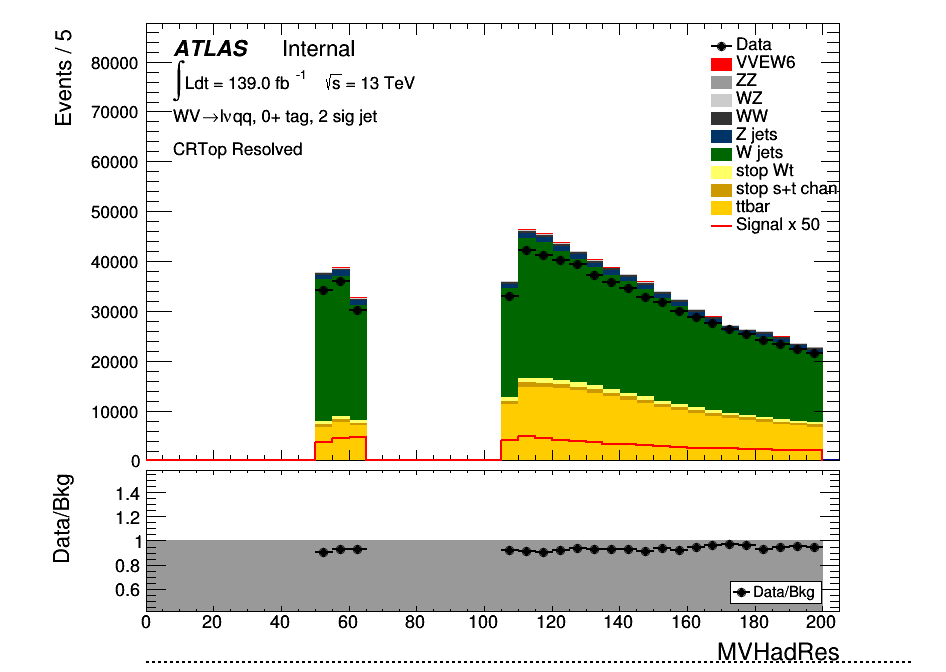
\includegraphics[width=\linewidth]{figures/1lep/CRPlots/C_0ptag2pjet_0ptv_CRVjet_MVHadRes_Lin.png}
        \caption{\emph{\olep, resolved WCR}}
    \end{subfigure}
    % You can add other subcaptions here if needed
    \caption{$m_{jj}$ plot in the sidebands in \zlep channel VCR (a), in \olep WCR (b) and \tlep channel ZCR (right).}
    \label{fig:1lep2lepMVHadResCR}
\end{figure}

%\begin{figure}[ht]
%    \begin{center}
%        \subfigure[]{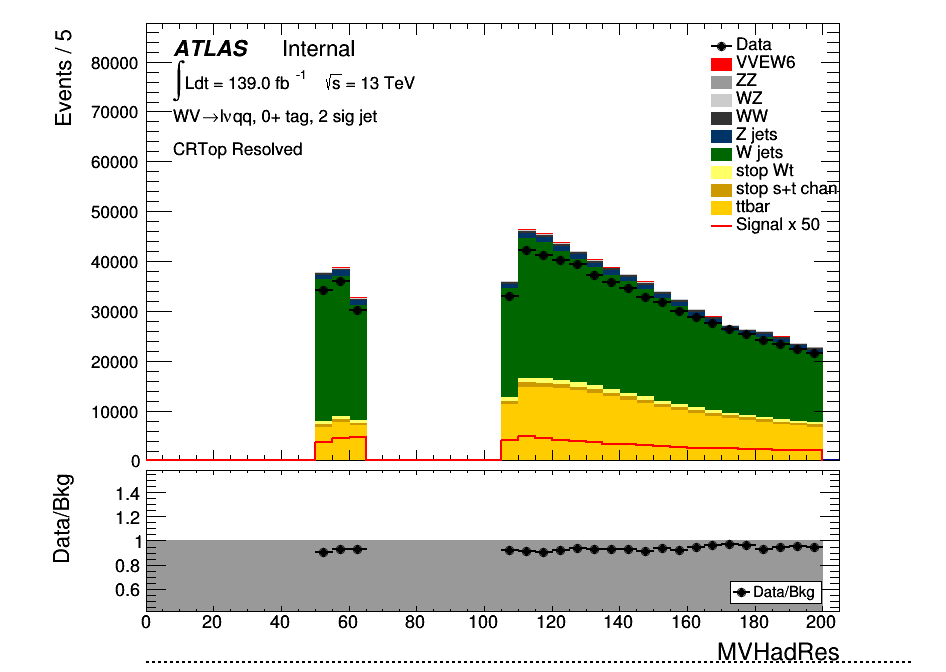
\includegraphics[width=0.3\textwidth]{figures/1lep/CRPlots/C_0ptag2pjet_0ptv_CRVjet_MVHadRes_Lin.png}}
%        \caption{ $m_{jj}$ plot in the sidebands in 1-lepton channel. }
%    \end{center}
%    \label{fig:1lepMVHadResCRVjet}
%\end{figure}

\subsubsection{$t\bar{t}$ CR (TCR)}
%\textbf{$t\bar{t}$ CR (TCR)}

%Two sets of the \ttbar CR (TR1 and TR2) can be used in this analysis.

In 1-lepton channel, TCR is defined by requiring at least one $b$-tagged jet instead of $b$-veto; distributions of the b-jets multiplicity for both resolved and merged regime are shown in figure \ref{fig:1lepNBjetsPresel}. 
%The purity of the $t\bar{t}$ background in this 
%region is 85\,\%. Signal contamination in both $W$+jets and $t\bar{t}$ control regions is negligible. The purity 
%of $W$+jets in WR is a bit poor, but the simultaneous fit to TR and WR makes it possible to determine the 
%normalization of $W$+jets correctly, thanks to high purity of $t\bar{t}$ in TR.

Since, the orthogonal cut is represented by the additional bjets in the event, 
the TCR correspond to mass window phase spaces, therefore, for the merged regime
TCR inherit the HP and LP splitting as for the SRs.

\begin{figure}[ht]
    \centering
    \begin{subfigure}{0.3\textwidth}
        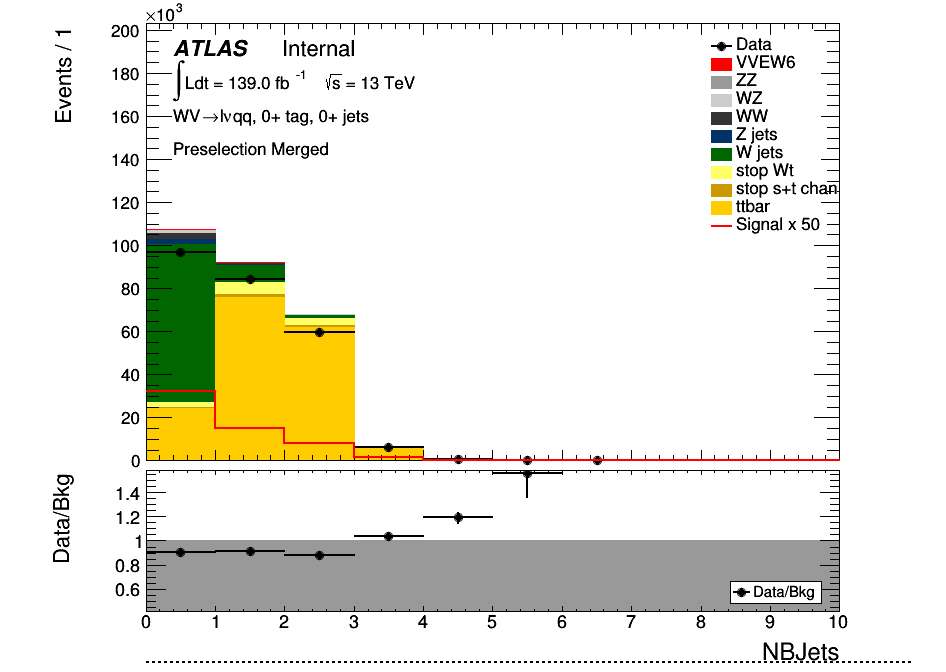
\includegraphics[width=\linewidth]{figures/1lep/CRPlots/C_0ptag0pjet_0ptv_Presel_Merged_NBJets_Lin.png}
        \caption{After merged preselection}
    \end{subfigure}
    \begin{subfigure}{0.3\textwidth}
        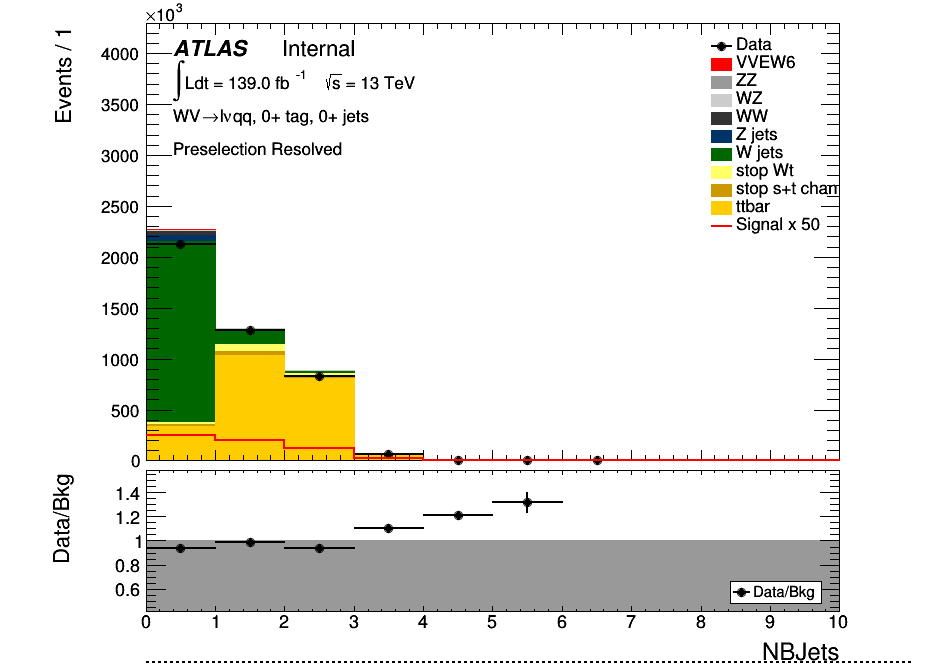
\includegraphics[width=\linewidth]{figures/1lep/CRPlots/C_0ptag0pjet_0ptv_Presel_Resolved_NBJets_Lin.png}
        \caption{After resolved preselection}
    \end{subfigure}
    \caption{Bjets multiplicity in the 1-lepton channel, after common preselection cuts have been applied.}
    \label{fig:1lepNBjetsPresel}
\end{figure}



%%%
\clearpage
\section{Signal and Background Cut-flows}
\clearpage
\subsubsection{Signal and background cut-flows}
\label{subsec:cutflows}

Cutflow Tables are presented for different signal regions.

\zlep: Figure~\ref{tab:0lepCutFlow}.
\olep: Figure~\ref{fig:1lepCutFlow}.
\tlep: 
Tables~\ref{tab:2lep_HPSR},
\ref{tab:2lep_LPSR},
\ref{tab:2lep_ResolvedSR},
\ref{tab:2lep_MergedCR}, and
\ref{tab:2lep_ResolvedCR}.

Tables
\ref{tab:PrefitYield_TCRHP_Per}-
\ref{tab:PrefitYield_TCRLP_Per}-
\ref{tab:PrefitYield_TCRRes_Per} (TCR)-
\ref{tab:PrefitYield_VCRMer_Per}-
\ref{tab:PrefitYield_WCRMer_Per}-
\ref{tab:PrefitYield_ZCRMer_Per}-
\ref{tab:PrefitYield_VCRRes_Per}-
\ref{tab:PrefitYield_WCRRes_Per}-
\ref{tab:PrefitYield_ZCRRes_Per} (VCR)-
\ref{tab:PrefitYield_0lepHPSR_Per}-
\ref{tab:PrefitYield_1lepHPSR_Per}-
\ref{tab:PrefitYield_2lepHPSR_Per} (HPSR)-
\ref{tab:PrefitYield_0lepLPSR_Per}-
\ref{tab:PrefitYield_1lepLPSR_Per}-
\ref{tab:PrefitYield_2lepLPSR_Per} (LPSR)-
\ref{tab:PrefitYield_0lepResSR_Per}-
\ref{tab:PrefitYield_1lepResSR_Per}-
\ref{tab:PrefitYield_2lepResSR_Per} (ResolvedSR)
show the final yields, in percentages, of the different CRs and SRs; 
the uncertainties account for statistical and systematic sources.


%%% 2-leptons channel
%%% HPSR 
\begin{table}[ht!]
\small
\caption{Cutflow table for HPSR region in \tlep channel. PassCommon cut refers to the lepton pre-selection and SFLetpons to the requirement to have SameFlavor leptons.}
\label{tab:2lep_HPSR}
\begin{center}
\resizebox{\textwidth}{!}{

 \begin{tabular}{ r ||  r  r  r  r  r  r  r  r  r  || r r r r r |}
 \ensuremath{\sqrt{s}=13 TeV}, \ensuremath{\mathcal{L}=139 fb^{-1}}  & W & WZ & WW & Z & ZZ & stopWtDilep & stops & stopt & ttbar & S & B & S/B & \ensuremath{S/\sqrt{B}}\tabularnewline
 \hline
All & 768630 & 118757 & 7549.85 & 2.69014e+07 & 75904.3 & 219335 & 1566.79 & 30086.3 & 3.4463e+06 & 8530.6 &3.15695e+07&0.000270216 & 1.51826\tabularnewline \hline
passCommon & 8949.67 & 73105.4 & 138.511 & 1.59613e+07 & 48170 & 22208.8 & 61.7359 & 1002.7 & 361153 & 3577.38&1.64761e+07&0.000217125 & 0.881328\tabularnewline \hline
TwoTagMerJets & 5430.67 & 41182 & 83.2249 & 9.38413e+06 & 24924.9 & 14016.8 & 33.1233 & 711.353 & 243694 & 2890.74&9.7142e+06&0.000297579 & 0.927483\tabularnewline \hline
PtTagMerJet1 & 4846.86 & 39715 & 80.198 & 7.66047e+06 & 23830.9 & 13522.8 & 31.7876 & 687.684 & 240045 & 2881.49 &7.98323e+06&0.000360943 & 1.01983\tabularnewline \hline
PtTagMerJet2 & 2692.05 & 26366.4 & 51.0517 & 3.74324e+06 & 14613 & 8652.04 & 19.427 & 455.492 & 180641 & 2527.77 &3.97673e+06&0.000635639 & 1.26758\tabularnewline \hline
AtLeastOneFatJet & 73.9896 & 1355.28 & 2.49747 & 54043.4 & 401.963 & 194.503 & 0.683082 & 9.52178 & 4071.51 & 190.792 &60153.4&0.00317176 & 0.777912\tabularnewline \hline
PtFatJet200 & 73.9896 & 1355.28 & 2.49747 & 54043.4 & 401.963 & 194.503 & 0.683082 & 9.52178 & 4071.51 & 190.792 &60153.4&0.00317176 & 0.777912\tabularnewline \hline
EtaFatJet2p0 & 73.9896 & 1355.28 & 2.49747 & 54043.4 & 401.963 & 194.503 & 0.683082 & 9.52178 & 4071.51 & 190.792 &60153.4&0.00317176 & 0.777912\tabularnewline \hline
dRL-eptonFatjet & 65.6967 & 1241.31 & 2.08247 & 50386.7 & 372.277 & 176.007 & 0.617677 & 8.85472 & 3270.23 & 177.47 &55523.8&0.0031963 & 0.753158\tabularnewline \hline
MFatJetLow & 26.3573 & 593.162 & 1.36814 & 17874.7 & 176.377 & 57.5099 & 0.147335 & 3.37462 & 1340.61 & 120.588 &20073.6&0.00600731 & 0.851124\tabularnewline \hline
SFLeptons & 8.29704 & 592.425 & 0.528064 & 17868.5 & 176.306 & 19.6953 & 0.0648612 & 1.36886 & 425.456 & 120.184 &19092.6&0.00629476 & 0.869786\tabularnewline \hline
MFatJet50 & 3.97632 & 321.546 & 0.150938 & 8269.29 & 98.0685 & 9.3015 & 0.0648612 & 0.426969 & 201.394 & 77.5594 &8904.22&0.00871041 & 0.821933\tabularnewline \hline
D2FatJet50 & 1.6553 & 164.963 & 0.150938 & 3032.68 & 52.9234 & 5.01844 & 0.0207499 & 0.246388 & 81.719 & 50.0044 & 3339.37&0.0149742 & 0.865317\tabularnewline \hline
NTrkFatJet50 & 1.24764 & 114.689 & 0.150938 & 1527.16 & 36.5107 & 2.48592 & 0.0207499 & 0.213116 & 41.1061 & 40.9103 &1723.59&0.0237356 & 0.985409\tabularnewline \hline
WZFatJet50 & 0.655411 & 112.269 & 0.150938 & 1469.7 & 35.6488 & 2.48592 & 0.0207499 & 0.213116 & 39.669 & 40.1491 &1660.82&0.0241743 & 0.985179\tabularnewline \hline
MTagMerJets400 & 0.608311 & 89.745 & 0.150938 & 1247.25 & 27.2269 & 2.34095 & 0.0207499 & 0.0789171 & 33.3017 & 37.6674 &1400.73&0.0268913 & 1.00644\tabularnewline \hline
\end{tabular}

}
\end{center}
\end{table}
%%
%%% LPSR 
\begin{table}[ht!]
\small
\caption{Cutflow table for LPSR region in \tlep channel}
\label{tab:2lep_LPSR}
\begin{center}
\resizebox{\textwidth}{!}{

 \begin{tabular}{ r ||  r  r  r  r  r  r  r  r  r  || r r r r r |}
 \ensuremath{\sqrt{s}=13 TeV}, \ensuremath{\mathcal{L}=139 fb^{-1}}  & W & WZ & WW & Z & ZZ & stopWtDilep & stops & stopt & ttbar &  S & B & S/B & \ensuremath{S/\sqrt{B}}\tabularnewline
 \hline
All & 768630 & 118757 & 7549.85 & 2.69014e+07 & 75904.3 & 219335 & 1566.79 & 30086.3 & 3.4463e+06 & 8530.6&3.15695e+07&0.000270216 & 1.51826\tabularnewline \hline
FailMergedSR50 & 768630 & 118667 & 7549.7 & 2.69001e+07 & 75877.1 & 219333 & 1566.77 & 30086.3 & 3.44627e+06 & 8492.93&3.15681e+07&0.000269035 & 1.51159\tabularnewline \hline
Trigger & 562963 & 108010 & 5681.35 & 2.40927e+07 & 69318 & 195862 & 1133.62 & 21873.2 & 3.02893e+06 & 7222.22 &2.80865e+07&0.000257142 & 1.36277\tabularnewline \hline
BothLepPt & 67751.3 & 90649.8 & 1147.71 & 2.07619e+07 & 59529.4 & 156592 & 304.094 & 4763.36 & 2.38282e+06 & 4798.78 &2.35255e+07&0.000203982 & 0.989376\tabularnewline \hline
LeadLepPt & 67452.8 & 90574.8 & 1141.41 & 2.0715e+07 & 59477 & 156269 & 301.881 & 4729.08 & 2.37606e+06 & 4792.64 &2.3471e+07&0.000204194 & 0.989256\tabularnewline \hline
MuonEtaLt2p5 & 66379 & 89424.2 & 1118.34 & 2.04089e+07 & 58762.6 & 155201 & 291.395 & 4617.26 & 2.3588e+06 & 4734.01 &2.31435e+07&0.00020455 & 0.984044\tabularnewline \hline
OSMuons & 65152 & 89398.7 & 1101.67 & 2.04087e+07 & 58761 & 155164 & 263.104 & 4354.02 & 2.35796e+06 & 4696.69 &2.31409e+07&0.000202961 & 0.976342\tabularnewline \hline
Mll & 8949.06 & 73015.6 & 138.36 & 1.596e+07 & 48142.8 & 22206.4 & 61.7151 & 1002.62 & 361120 & 3539.71 &1.64747e+07&0.000214858 & 0.872086\tabularnewline \hline
TwoTagMerJets & 5430.07 & 41092.3 & 83.0739 & 9.38288e+06 & 24897.7 & 14014.5 & 33.1025 & 711.274 & 243660 & 2853.07&9.7128e+06&0.000293744 & 0.915463\tabularnewline \hline
PtTagMerJet1 & 4846.25 & 39625.3 & 80.047 & 7.65922e+06 & 23803.7 & 13520.5 & 31.7668 & 687.605 & 240012  & 2843.82&7.98183e+06&0.000356287 & 1.00659\tabularnewline \hline
PtTagMerJet2 & 2691.44 & 26276.6 & 50.9008 & 3.74199e+06 & 14585.8 & 8649.7 & 19.4063 & 455.413 & 180607  & 2490.1&3.97533e+06&0.000626388 & 1.24891\tabularnewline \hline
AtLeastOneFatJet & 73.3813 & 1265.54 & 2.34653 & 52796.2 & 374.736 & 192.162 & 0.662332 & 9.44287 & 4038.21 & 153.125&58752.7&0.00260626 & 0.63173\tabularnewline \hline
PtFatJet200 & 73.3813 & 1265.54 & 2.34653 & 52796.2 & 374.736 & 192.162 & 0.662332 & 9.44287 & 4038.21  & 153.125&58752.7&0.00260626 & 0.63173\tabularnewline \hline
EtaFatJet2p0 & 73.3813 & 1265.54 & 2.34653 & 52796.2 & 374.736 & 192.162 & 0.662332 & 9.44287 & 4038.21  & 153.125&58752.7&0.00260626 & 0.63173\tabularnewline \hline
dRLeptonFatjet & 65.0884 & 1151.57 & 1.93153 & 49139.4 & 345.05 & 173.666 & 0.596927 & 8.7758 & 3236.93  & 139.803&54123&0.00258306 & 0.600932\tabularnewline \hline
MFatJetLow & 25.749 & 503.417 & 1.2172 & 16627.4 & 149.15 & 55.1689 & 0.126585 & 3.29571 & 1307.31 & 82.921 &18672.9&0.00444072 & 0.606818\tabularnewline \hline
SFLeptons & 7.68872 & 502.68 & 0.377126 & 16621.2 & 149.079 & 17.3543 & 0.0441112 & 1.28994 & 392.155 & 82.5162 &17691.9&0.00466406 & 0.620371\tabularnewline \hline
MFatJet80 & 4.50972 & 305.264 & 0.0531649 & 9708.43 & 92.5334 & 9.79512 & 0.0441112 & 0.8637 & 230.263 & 53.3019 &10351.8&0.00514907 & 0.523884\tabularnewline \hline
D2FatJet80 & 3.0742 & 220.826 & 0 & 6606.32 & 67.506 & 8.12447 & 0 & 0.652429 & 167.653 & 40.3886 &7074.16&0.00570932 & 0.480199\tabularnewline \hline
NTrkFatJet80 & 1.80329 & 175.492 & 0 & 4548.12 & 53.5843 & 4.93659 & 0 & 0.58877 & 106.823 & 36.0306 &4891.35&0.0073662 & 0.515178\tabularnewline \hline
WZFatJet80 & 1.80329 & 170.838 & 0 & 4389.69 & 52.4945 & 4.55232 & 0 & 0.58877 & 103.266 & 35.429 &4723.23&0.007501 & 0.515512\tabularnewline \hline
MTagMerJets400 & 1.67793 & 123.578 & 0 & 3541.1 & 35.3674 & 3.94765 & 0 & 0.454571 & 80.232 & 30.8227 &3786.36&0.00814046 & 0.50091\tabularnewline \hline
\end{tabular}

}
\end{center}
\end{table}
%
%% Resolved SR 
\begin{table}[ht!]
\small
\caption{Cutflow table for Resolved SR region in \tlep channel}
\label{tab:2lep_ResolvedSR}
\begin{center}
\resizebox{\textwidth}{!}{

 \begin{tabular}{ r ||  r  r  r  r  r  r  r  r  r  r || r r r r r |}
 \ensuremath{\sqrt{s}=13 TeV}, \ensuremath{\mathcal{L}=139 fb^{-1}}  & W & WZ & WW & Z & ZZ & stopWtDilep & stops & stopt & ttbar & S  & B & S/B & \ensuremath{S/\sqrt{B}}\tabularnewline
 \hline
All & 768630 & 118757 & 7549.85 & 2.69014e+07 & 75904.3 & 219335 & 1566.79 & 30086.3 & 3.4463e+06 & 8530.6 &3.15695e+07&0.000270216 & 1.51826\tabularnewline \hline
FailMergedSR50 & 768630 & 118667 & 7549.7 & 2.69001e+07 & 75877.1 & 219333 & 1566.77 & 30086.3 & 3.44627e+06 & 8492.93&3.15681e+07&0.000269035 & 1.51159\tabularnewline \hline
FailMergedSR80 & 768628 & 118544 & 7549.7 & 2.68966e+07 & 75841.7 & 219329 & 1566.77 & 30085.8 & 3.44619e+06 & 8462.11&3.15643e+07&0.000268091 & 1.50619\tabularnewline \hline
Trigger & 562961 & 107887 & 5681.35 & 2.40892e+07 & 69282.7 & 195858 & 1133.62 & 21872.7 & 3.02885e+06 & 7191.4 &2.80827e+07&0.000256079 & 1.35704\tabularnewline \hline
BothLepPt & 67749.6 & 90526.2 & 1147.71 & 2.07584e+07 & 59494 & 156588 & 304.094 & 4762.91 & 2.38274e+06 & 4767.96 &2.35217e+07&0.000202705 & 0.983101\tabularnewline \hline
LeadLepPt & 67451.1 & 90451.2 & 1141.41 & 2.07115e+07 & 59441.7 & 156265 & 301.881 & 4728.63 & 2.37598e+06 & 4761.82 &2.34672e+07&0.000202913 & 0.982973\tabularnewline \hline
MuonEtaLt2p5 & 66377.3 & 89300.6 & 1118.34 & 2.04053e+07 & 58727.3 & 155197 & 291.395 & 4616.81 & 2.35872e+06 & 4703.18 &2.31397e+07&0.000203252 & 0.977717\tabularnewline \hline
OSMuons & 65150.4 & 89275.1 & 1101.67 & 2.04052e+07 & 58725.7 & 155160 & 263.104 & 4353.56 & 2.35788e+06 & 4665.87 &2.31371e+07&0.000201662 & 0.970014\tabularnewline \hline
Mll & 8947.38 & 72892.1 & 138.36 & 1.59565e+07 & 48107.4 & 22202.5 & 61.7151 & 1002.17 & 361040 & 3508.89 &1.64709e+07&0.000213036 & 0.864591\tabularnewline \hline
TwoTagResJets & 5428.39 & 40968.7 & 83.0739 & 9.37934e+06 & 24862.3 & 14010.5 & 33.1025 & 710.82 & 243580 & 2822.25&9.70902e+06&0.000290684 & 0.90575\tabularnewline \hline
PtTagResJet1 & 4844.57 & 39501.7 & 80.047 & 7.65568e+06 & 23768.3 & 13516.5 & 31.7668 & 687.15 & 239932 & 2813 &7.97804e+06&0.000352593 & 0.995913\tabularnewline \hline
PtTagResJet2 & 2689.76 & 26153.1 & 50.9008 & 3.73845e+06 & 14550.4 & 8645.75 & 19.4063 & 454.958 & 180527 & 2459.28 &3.97154e+06&0.000619224 & 1.23404\tabularnewline \hline
TwoSigJets & 1224.28 & 15670.2 & 27.3266 & 1.35255e+06 & 7188.69 & 3383.22 & 6.95563 & 193.559 & 97769.1 & 1983.71 &1.47801e+06&0.00134215 & 1.6317\tabularnewline \hline
PtSignalJet1 & 895.835 & 12934.8 & 23.2614 & 908980 & 5628.78 & 2675.5 & 5.30779 & 148.163 & 83593 & 1796.12 &1.01488e+06&0.00176978 & 1.7829\tabularnewline \hline
PtSignalJet2 & 895.835 & 12934.8 & 23.2614 & 908980 & 5628.78 & 2675.5 & 5.30779 & 148.163 & 83593 & 1796.12 &1.01488e+06&0.00176978 & 1.7829\tabularnewline \hline
MVHadResLow & 786.438 & 11881.2 & 21.6767 & 797009 & 5103.81 & 2390.64 & 4.78611 & 135.01 & 75903.6 & 1690.66&893237&0.00189273 & 1.78884\tabularnewline \hline
SFLeptons & 238.494 & 11869.8 & 8.04294 & 796752 & 5102.21 & 738.483 & 1.51008 & 43.6911 & 23211.2 & 1673.08&837966&0.0019966 & 1.82769\tabularnewline \hline
MVHadRes & 82.6204 & 3972.79 & 2.81781 & 251182 & 1838.78 & 204.164 & 0.436533 & 12.379 & 6566.27 & 782.652&263862&0.00296614 & 1.52363\tabularnewline \hline
MTagResJets400 & 36.9849 & 1922.17 & 1.59711 & 139844 & 814.46 & 100.109 & 0.263526 & 9.07562 & 3048.05 & 581.914&145777&0.00399182 & 1.5241\tabularnewline \hline
passMjjjRes & 15.7732 & 479.481 & 0.603948 & 37458.8 & 189.746 & 32.6127 & 0.0863601 & 3.17091 & 888.228 & 177.763&39068.5&0.00455005 & 0.899351\tabularnewline \hline
\end{tabular}

}
\end{center}
\end{table}

%% Merged CR 
\begin{table}[ht!]
\small
\caption{Cutflow table for Merged CR region in \tlep channel}
\label{tab:2lep_MergedCR}
\begin{center}
\resizebox{\textwidth}{!}{
 \begin{tabular}{ r ||  r  r  r  r  r  r  r  r  r  r || r r r r r |}
 \ensuremath{\sqrt{s}=13 TeV}, \ensuremath{\mathcal{L}=139 fb^{-1}}  & ttbar & ZZ & WW & WZ & W & stopWtDilep & stops & stopt & Z & S & B & S/B & \ensuremath{S/\sqrt{B}}\tabularnewline
 \hline
All & 3.4463e+06 & 75905.5 & 7549.85 & 118761 & 768630 & 219335 & 1566.79 & 30086.3 & 2.69016e+07 & 8532.15 &3.15697e+07&0.000270264 & 1.51853\tabularnewline \hline
FailMergedSR50 & 3.44626e+06 & 75878.3 & 7549.7 & 118672 & 768630 & 219333 & 1566.77 & 30086.3 & 2.69003e+07 & 8494.48&3.15683e+07&0.000269083 & 1.51186\tabularnewline \hline
FailMergedSR80 & 3.44618e+06 & 75842.9 & 7549.7 & 118548 & 768628 & 219329 & 1566.77 & 30085.8 & 2.68968e+07 & 8463.66&3.15645e+07&0.000268138 & 1.50646\tabularnewline \hline
FailResolvedSR & 3.44314e+06 & 75028.5 & 7548.1 & 116626 & 768591 & 219229 & 1566.51 & 30076.7 & 2.6757e+07 & 7881.75&3.14188e+07&0.000250861 & 1.40614\tabularnewline \hline
passMerged & 1188.84 & 99.8369 & 1.21642 & 329.927 & 22.442 & 49.5988 & 0.126065 & 2.63054 & 11199.6 & 39.5744 &12894.2&0.00306916 & 0.348511\tabularnewline \hline
SFLeptons & 273.684 & 99.7661 & 0.376343 & 329.189 & 4.38175 & 11.7842 & 0.0435912 & 0.624779 & 11193.4 & 39.1696 &11913.2&0.0032879 & 0.358868\tabularnewline \hline
MTagMerJets400 & 207.59 & 68.1131 & 0.376343 & 234.978 & 3.30903 & 7.99553 & 0.0435912 & 0.448283 & 8747.54 & 31.3438 &9270.39&0.00338107 & 0.325539\tabularnewline \hline
FailWZFatJet80 & 207.59 & 68.1131 & 0.376343 & 234.978 & 3.30903 & 7.99553 & 0.0435912 & 0.448283 & 8747.54 & 31.3438 &9270.39&0.00338107 & 0.325539\tabularnewline \hline
\end{tabular}
}
\end{center}
\end{table}
%% Resolved CRFid 
\begin{table}[ht!]
\small
\caption{Cutflow table for Resolved CR region in \tlep channel}
\label{tab:2lep_ResolvedCR}
\begin{center}
\resizebox{\textwidth}{!}{
 \begin{tabular}{ r ||  r  r  r  r  r  r  r  r  r  r || r r r r r |}
 \ensuremath{\sqrt{s}=13 TeV}, \ensuremath{\mathcal{L}=139 fb^{-1}}  & ttbar & ZZ & WW & WZ & W & stopWtDilep & stops & stopt & Z &  S & B & S/B & \ensuremath{S/\sqrt{B}}\tabularnewline
 \hline
All & 3.4463e+06 & 75905.5 & 7549.85 & 118761 & 768630 & 219335 & 1566.79 & 30086.3 & 2.69016e+07 & 8532.15 &3.15697e+07&0.000270264 & 1.51853\tabularnewline \hline
FailMergedSR50 & 3.44626e+06 & 75878.3 & 7549.7 & 118672 & 768630 & 219333 & 1566.77 & 30086.3 & 2.69003e+07 & 8494.48&3.15683e+07&0.000269083 & 1.51186\tabularnewline \hline
FailMergedSR80 & 3.44618e+06 & 75842.9 & 7549.7 & 118548 & 768628 & 219329 & 1566.77 & 30085.8 & 2.68968e+07 & 8463.66&3.15645e+07&0.000268138 & 1.50646\tabularnewline \hline
FailResolvedSR & 3.44314e+06 & 75028.5 & 7548.1 & 116626 & 768591 & 219229 & 1566.51 & 30076.7 & 2.6757e+07 & 7881.75&3.14188e+07&0.000250861 & 1.40614\tabularnewline \hline
FailMergedCR & 3.44293e+06 & 74960.3 & 7547.72 & 116391 & 768588 & 219221 & 1566.46 & 30076.3 & 2.67482e+07 & 7850.4&3.14095e+07&0.000249937 & 1.40075\tabularnewline \hline
passResolved & 72648.8 & 4223.49 & 19.7025 & 9732.45 & 746.638 & 2282.95 & 4.47847 & 125.48 & 648996 & 1080.44 &738780&0.00146247 & 1.25702\tabularnewline \hline
SFLeptons & 19956.4 & 4221.89 & 6.06871 & 9721.07 & 198.693 & 630.797 & 1.20244 & 34.1617 & 648739 & 1062.86 &683509&0.00155501 & 1.2856\tabularnewline \hline
FailMVhadRes & 16438.2 & 3197.57 & 4.84801 & 7670.44 & 153.058 & 526.741 & 1.02944 & 30.8583 & 537401 & 862.124 &565424&0.00152474 & 1.14652\tabularnewline \hline
\end{tabular}
}
\end{center}
\end{table}

%%%%%%%%%%%%%%%%%%%%%%%%%%
%     1 Lep Channel Cutflows
\begin{figure}[ht]
    \centering
    \begin{subfigure}{\textwidth}
        \resizebox{\textwidth}{!}{ \begin{tabular}{ r ||  r  r  r  r  r  r || r r r |} 
 \ensuremath{\sqrt{s}=13 TeV}, \ensuremath{\mathcal{L}=139.0 fb^{-1}}  & Wjets & Zjets & Diboson & ttbar & singletop & EW6Signal& Data & Data/MC & Total BG MC \tabularnewline 
 \hline 
All & 55324079.19$\pm$26220.39 & 4876715.84$\pm$6254.47 & 780707.22$\pm$433.93 & 13223935.55$\pm$1379.85 & 2027933.67$\pm$451.68 & 73297.23$\pm$44.50 & 95607223.00$\pm$9777.89 & 1.25 & 76306668.71$\pm$26998.62\tabularnewline \hline 
pass Preselection & 45948511.98$\pm$23483.02 & 4141626.70$\pm$5740.56 & 658544.95$\pm$388.63 & 10779287.74$\pm$1242.33 & 1658253.97$\pm$409.05 & 59096.53$\pm$39.62 & 76693252.00$\pm$8757.47 & 1.21 & 63245321.88$\pm$24213.01\tabularnewline \hline 
TagJet30Merged & 17153016.15$\pm$12030.83 & 1527403.58$\pm$3000.67 & 274751.78$\pm$241.29 & 6212629.30$\pm$942.65 & 852949.30$\pm$289.70 & 37724.74$\pm$30.84 & 29424546.00$\pm$5424.44 & 1.13 & 26058474.86$\pm$12440.92\tabularnewline \hline 
OneLargeJet & 456643.60$\pm$457.36 & 35082.45$\pm$81.56 & 17871.04$\pm$52.83 & 399654.20$\pm$238.55 & 41477.26$\pm$67.97 & 2784.08$\pm$6.94 & 946535.00$\pm$972.90 & 0.99 & 953512.63$\pm$529.34\tabularnewline \hline 
MET 80 & 223921.14$\pm$319.59 & 7675.53$\pm$46.12 & 9077.57$\pm$38.44 & 234251.21$\pm$183.80 & 25183.28$\pm$53.73 & 1619.01$\pm$5.37 & 472216.00$\pm$687.18 & 0.94 & 501727.74$\pm$377.41\tabularnewline \hline 
Mjj400Merged & 190006.61$\pm$293.87 & 6624.64$\pm$42.69 & 7773.93$\pm$35.44 & 194133.57$\pm$167.46 & 21522.24$\pm$49.51 & 1459.31$\pm$4.97 & 394311.00$\pm$627.94 & 0.94 & 421520.30$\pm$346.35\tabularnewline \hline 
fatJWP50 & 4843.61$\pm$43.06 & 189.04$\pm$5.93 & 742.44$\pm$11.23 & 22981.84$\pm$57.68 & 2474.95$\pm$18.07 & 382.07$\pm$2.44 & 26088.00$\pm$161.52 & 0.83 & 31613.93$\pm$75.33\tabularnewline \hline 
MerTagBJetVeto & 4535.60$\pm$42.56 & 172.00$\pm$5.82 & 699.48$\pm$10.95 & 8713.76$\pm$35.56 & 853.14$\pm$10.51 & 282.80$\pm$1.77 & 13180.00$\pm$114.80 & 0.86 & 15256.77$\pm$57.82\tabularnewline \hline 
\end{tabular}
}
        \caption{SR High Purity Merged}
    \end{subfigure}
    \begin{subfigure}{\textwidth}
        \resizebox{\textwidth}{!}{ \begin{tabular}{ r ||  r  r  r  r  r  r || r r r |} 
 \ensuremath{\sqrt{s}=13 TeV}, \ensuremath{\mathcal{L}=139.0 fb^{-1}}  & Wjets & Zjets & Diboson & ttbar & singletop & EW6Signal& Data & Data/MC & Total BG MC \tabularnewline 
 \hline 
All & 55324079.19$\pm$26220.39 & 4876715.84$\pm$6254.47 & 780707.22$\pm$433.93 & 13223935.55$\pm$1379.85 & 2027933.67$\pm$451.68 & 73297.23$\pm$44.50 & 95607223.00$\pm$9777.89 & 1.25 & 76306668.71$\pm$26998.62\tabularnewline \hline 
pass Preselection & 45948511.98$\pm$23483.02 & 4141626.70$\pm$5740.56 & 658544.95$\pm$388.63 & 10779287.74$\pm$1242.33 & 1658253.97$\pm$409.05 & 59096.53$\pm$39.62 & 76693252.00$\pm$8757.47 & 1.21 & 63245321.88$\pm$24213.01\tabularnewline \hline 
TagJet30Merged & 17153016.15$\pm$12030.83 & 1527403.58$\pm$3000.67 & 274751.78$\pm$241.29 & 6212629.30$\pm$942.65 & 852949.30$\pm$289.70 & 37724.74$\pm$30.84 & 29424546.00$\pm$5424.44 & 1.13 & 26058474.86$\pm$12440.92\tabularnewline \hline 
OneLargeJet & 456643.60$\pm$457.36 & 35082.45$\pm$81.56 & 17871.04$\pm$52.83 & 399654.20$\pm$238.55 & 41477.26$\pm$67.97 & 2784.08$\pm$6.94 & 946535.00$\pm$972.90 & 0.99 & 953512.63$\pm$529.34\tabularnewline \hline 
MET 80 & 223921.14$\pm$319.59 & 7675.53$\pm$46.12 & 9077.57$\pm$38.44 & 234251.21$\pm$183.80 & 25183.28$\pm$53.73 & 1619.01$\pm$5.37 & 472216.00$\pm$687.18 & 0.94 & 501727.74$\pm$377.41\tabularnewline \hline 
Mjj400Merged & 190006.61$\pm$293.87 & 6624.64$\pm$42.69 & 7773.93$\pm$35.44 & 194133.57$\pm$167.46 & 21522.24$\pm$49.51 & 1459.31$\pm$4.97 & 394311.00$\pm$627.94 & 0.94 & 421520.30$\pm$346.35\tabularnewline \hline 
fatJWP80 & 18753.40$\pm$99.47 & 708.62$\pm$14.52 & 1627.81$\pm$16.40 & 52081.37$\pm$86.73 & 5013.06$\pm$25.24 & 646.11$\pm$3.21 & 68583.00$\pm$261.88 & 0.87 & 78830.37$\pm$136.18\tabularnewline \hline 
MerTagBJetVeto & 17624.00$\pm$98.66 & 649.34$\pm$14.42 & 1523.27$\pm$15.96 & 20132.76$\pm$53.99 & 1894.07$\pm$15.36 & 475.10$\pm$2.33 & 37412.00$\pm$193.42 & 0.88 & 42298.53$\pm$115.56\tabularnewline \hline 
\end{tabular}
}
        \caption{SR Low Purity Merged}
    \end{subfigure}
    \begin{subfigure}{\textwidth}
        \resizebox{\textwidth}{!}{ \begin{tabular}{ r ||  r  r  r  r  r  r || r r r |} 
 \ensuremath{\sqrt{s}=13 TeV}, \ensuremath{\mathcal{L}=139.0 fb^{-1}}  & Wjets & Zjets & Diboson & ttbar & singletop & EW6Signal& Data & Data/MC & Total BG MC \tabularnewline 
 \hline 
All & 55324079.19$\pm$26220.39 & 4876715.84$\pm$6254.47 & 780707.22$\pm$433.93 & 13223935.55$\pm$1379.85 & 2027933.67$\pm$451.68 & 73297.23$\pm$44.50 & 95607223.00$\pm$9777.89 & 1.25 & 76306668.71$\pm$26998.62\tabularnewline \hline 
pass Preselection & 45948511.98$\pm$23483.02 & 4141626.70$\pm$5740.56 & 658544.95$\pm$388.63 & 10779287.74$\pm$1242.33 & 1658253.97$\pm$409.05 & 59096.53$\pm$39.62 & 76693252.00$\pm$8757.47 & 1.21 & 63245321.88$\pm$24213.01\tabularnewline \hline 
MET 80 & 11811513.88$\pm$10296.89 & 343801.40$\pm$1316.97 & 197270.06$\pm$212.69 & 4595534.91$\pm$811.83 & 604990.61$\pm$251.01 & 23100.14$\pm$24.19 & 18079828.00$\pm$4252.04 & 1.03 & 17576211.00$\pm$10417.69\tabularnewline \hline 
2tagJets & 7384002.43$\pm$8123.45 & 229146.75$\pm$1085.03 & 122263.82$\pm$161.21 & 3408543.10$\pm$698.83 & 429882.24$\pm$209.68 & 17938.71$\pm$21.05 & 11576602.00$\pm$3402.44 & 1.00 & 11591777.05$\pm$8229.61\tabularnewline \hline 
TagJet30Resolved & 4935873.63$\pm$5746.83 & 157880.80$\pm$757.11 & 92357.75$\pm$137.98 & 2733218.42$\pm$626.25 & 332414.15$\pm$184.45 & 15190.70$\pm$19.07 & 8190984.00$\pm$2861.99 & 0.99 & 8266935.47$\pm$5834.80\tabularnewline \hline 
Mjj400Resolved & 2521707.37$\pm$3705.72 & 92280.44$\pm$569.88 & 49360.73$\pm$97.00 & 1325962.02$\pm$437.12 & 179625.70$\pm$132.91 & 9573.45$\pm$13.96 & 4047289.00$\pm$2011.79 & 0.97 & 4178509.71$\pm$3778.29\tabularnewline \hline 
TwoSigJets & 1324404.99$\pm$2178.87 & 53368.18$\pm$373.72 & 37727.53$\pm$81.75 & 1215474.13$\pm$418.30 & 127876.33$\pm$116.07 & 8024.12$\pm$12.89 & 2594368.00$\pm$1610.70 & 0.94 & 2766875.28$\pm$2254.43\tabularnewline \hline 
sigJJmassWindow & 279163.62$\pm$1061.43 & 11185.36$\pm$184.93 & 8858.94$\pm$40.34 & 290270.24$\pm$204.33 & 29647.38$\pm$56.76 & 3033.89$\pm$7.71 & 578706.00$\pm$760.73 & 0.93 & 622159.42$\pm$1098.86\tabularnewline \hline 
ResTagBJetVeto & 268041.47$\pm$1057.95 & 10642.78$\pm$184.52 & 8385.17$\pm$39.51 & 125600.54$\pm$134.32 & 15933.82$\pm$40.50 & 2078.05$\pm$5.54 & 397274.00$\pm$630.30 & 0.92 & 430681.81$\pm$1083.78\tabularnewline \hline 
Mjjj220 & 75772.32$\pm$503.07 & 2839.55$\pm$85.65 & 2381.19$\pm$21.22 & 17804.30$\pm$50.98 & 4157.23$\pm$19.73 & 976.09$\pm$3.16 & 99146.00$\pm$314.87 & 0.95 & 103930.68$\pm$513.68\tabularnewline \hline 
\end{tabular}
}
        \caption{SR Resolved}
    \end{subfigure}
    \begin{subfigure}{\textwidth}
        \resizebox{\textwidth}{!}{ \begin{tabular}{ r ||  r  r  r  r  r  r || r r r |} 
 \ensuremath{\sqrt{s}=13 TeV}, \ensuremath{\mathcal{L}=139.0 fb^{-1}}  & Wjets & Zjets & Diboson & ttbar & singletop & EW6Signal& Data & Data/MC & Total BG MC \tabularnewline 
 \hline 
All & 55324079.19$\pm$26220.39 & 4876715.84$\pm$6254.47 & 780707.22$\pm$433.93 & 13223935.55$\pm$1379.85 & 2027933.67$\pm$451.68 & 73297.23$\pm$44.50 & 95607223.00$\pm$9777.89 & 1.25 & 76306668.71$\pm$26998.62\tabularnewline \hline 
pass Preselection & 45948511.98$\pm$23483.02 & 4141626.70$\pm$5740.56 & 658544.95$\pm$388.63 & 10779287.74$\pm$1242.33 & 1658253.97$\pm$409.05 & 59096.53$\pm$39.62 & 76693252.00$\pm$8757.47 & 1.21 & 63245321.88$\pm$24213.01\tabularnewline \hline 
TagJet30Merged & 17153016.15$\pm$12030.83 & 1527403.58$\pm$3000.67 & 274751.78$\pm$241.29 & 6212629.30$\pm$942.65 & 852949.30$\pm$289.70 & 37724.74$\pm$30.84 & 29424546.00$\pm$5424.44 & 1.13 & 26058474.86$\pm$12440.92\tabularnewline \hline 
OneLargeJet & 456643.60$\pm$457.36 & 35082.45$\pm$81.56 & 17871.04$\pm$52.83 & 399654.20$\pm$238.55 & 41477.26$\pm$67.97 & 2784.08$\pm$6.94 & 946535.00$\pm$972.90 & 0.99 & 953512.63$\pm$529.34\tabularnewline \hline 
MET 80 & 223921.14$\pm$319.59 & 7675.53$\pm$46.12 & 9077.57$\pm$38.44 & 234251.21$\pm$183.80 & 25183.28$\pm$53.73 & 1619.01$\pm$5.37 & 472216.00$\pm$687.18 & 0.94 & 501727.74$\pm$377.41\tabularnewline \hline 
Mjj400Merged & 190006.61$\pm$293.87 & 6624.64$\pm$42.69 & 7773.93$\pm$35.44 & 194133.57$\pm$167.46 & 21522.24$\pm$49.51 & 1459.31$\pm$4.97 & 394311.00$\pm$627.94 & 0.94 & 421520.30$\pm$346.35\tabularnewline \hline 
fatJWP50 & 4843.61$\pm$43.06 & 189.04$\pm$5.93 & 742.44$\pm$11.23 & 22981.84$\pm$57.68 & 2474.95$\pm$18.07 & 382.07$\pm$2.44 & 26088.00$\pm$161.52 & 0.83 & 31613.93$\pm$75.33\tabularnewline \hline 
OneBJet & 308.01$\pm$6.58 & 17.04$\pm$1.16 & 42.96$\pm$2.52 & 14268.08$\pm$45.41 & 1621.80$\pm$14.69 & 99.28$\pm$1.68 & 12908.00$\pm$113.61 & 0.79 & 16357.16$\pm$48.29\tabularnewline \hline 
\end{tabular}
}
        \caption{TopCR High Purity Merged}
    \end{subfigure}
    \begin{subfigure}{\textwidth}
        \resizebox{\textwidth}{!}{ \begin{tabular}{ r ||  r  r  r  r  r  r || r r r |} 
 \ensuremath{\sqrt{s}=13 TeV}, \ensuremath{\mathcal{L}=139.0 fb^{-1}}  & Wjets & Zjets & Diboson & ttbar & singletop & EW6Signal& Data & Data/MC & Total BG MC \tabularnewline 
 \hline 
All & 55324079.19$\pm$26220.39 & 4876715.84$\pm$6254.47 & 780707.22$\pm$433.93 & 13223935.55$\pm$1379.85 & 2027933.67$\pm$451.68 & 73297.23$\pm$44.50 & 95607223.00$\pm$9777.89 & 1.25 & 76306668.71$\pm$26998.62\tabularnewline \hline 
pass Preselection & 45948511.98$\pm$23483.02 & 4141626.70$\pm$5740.56 & 658544.95$\pm$388.63 & 10779287.74$\pm$1242.33 & 1658253.97$\pm$409.05 & 59096.53$\pm$39.62 & 76693252.00$\pm$8757.47 & 1.21 & 63245321.88$\pm$24213.01\tabularnewline \hline 
TagJet30Merged & 17153016.15$\pm$12030.83 & 1527403.58$\pm$3000.67 & 274751.78$\pm$241.29 & 6212629.30$\pm$942.65 & 852949.30$\pm$289.70 & 37724.74$\pm$30.84 & 29424546.00$\pm$5424.44 & 1.13 & 26058474.86$\pm$12440.92\tabularnewline \hline 
OneLargeJet & 456643.60$\pm$457.36 & 35082.45$\pm$81.56 & 17871.04$\pm$52.83 & 399654.20$\pm$238.55 & 41477.26$\pm$67.97 & 2784.08$\pm$6.94 & 946535.00$\pm$972.90 & 0.99 & 953512.63$\pm$529.34\tabularnewline \hline 
MET 80 & 223921.14$\pm$319.59 & 7675.53$\pm$46.12 & 9077.57$\pm$38.44 & 234251.21$\pm$183.80 & 25183.28$\pm$53.73 & 1619.01$\pm$5.37 & 472216.00$\pm$687.18 & 0.94 & 501727.74$\pm$377.41\tabularnewline \hline 
Mjj400Merged & 190006.61$\pm$293.87 & 6624.64$\pm$42.69 & 7773.93$\pm$35.44 & 194133.57$\pm$167.46 & 21522.24$\pm$49.51 & 1459.31$\pm$4.97 & 394311.00$\pm$627.94 & 0.94 & 421520.30$\pm$346.35\tabularnewline \hline 
fatJWP80 & 18753.40$\pm$99.47 & 708.62$\pm$14.52 & 1627.81$\pm$16.40 & 52081.37$\pm$86.73 & 5013.06$\pm$25.24 & 646.11$\pm$3.21 & 68583.00$\pm$261.88 & 0.87 & 78830.37$\pm$136.18\tabularnewline \hline 
OneBJet & 1129.41$\pm$12.69 & 59.28$\pm$1.67 & 104.54$\pm$3.78 & 31948.61$\pm$67.88 & 3118.99$\pm$20.03 & 171.01$\pm$2.21 & 31171.00$\pm$176.55 & 0.85 & 36531.84$\pm$72.05\tabularnewline \hline 
\end{tabular}
}
        \caption{TopCR Low Purity Merged}
    \end{subfigure}
    \begin{subfigure}{\textwidth}
        \resizebox{\textwidth}{!}{ \begin{tabular}{ r ||  r  r  r  r  r  r || r r r |} 
 \ensuremath{\sqrt{s}=13 TeV}, \ensuremath{\mathcal{L}=139.0 fb^{-1}}  & Wjets & Zjets & Diboson & ttbar & singletop & EW6Signal& Data & Data/MC & Total BG MC \tabularnewline 
 \hline 
All & 55324079.19$\pm$26220.39 & 4876715.84$\pm$6254.47 & 780707.22$\pm$433.93 & 13223935.55$\pm$1379.85 & 2027933.67$\pm$451.68 & 73297.23$\pm$44.50 & 95607223.00$\pm$9777.89 & 1.25 & 76306668.71$\pm$26998.62\tabularnewline \hline 
pass Preselection & 45948511.98$\pm$23483.02 & 4141626.70$\pm$5740.56 & 658544.95$\pm$388.63 & 10779287.74$\pm$1242.33 & 1658253.97$\pm$409.05 & 59096.53$\pm$39.62 & 76693252.00$\pm$8757.47 & 1.21 & 63245321.88$\pm$24213.01\tabularnewline \hline 
MET 80 & 11811513.88$\pm$10296.89 & 343801.40$\pm$1316.97 & 197270.06$\pm$212.69 & 4595534.91$\pm$811.83 & 604990.61$\pm$251.01 & 23100.14$\pm$24.19 & 18079828.00$\pm$4252.04 & 1.03 & 17576211.00$\pm$10417.69\tabularnewline \hline 
2tagJets & 7384002.43$\pm$8123.45 & 229146.75$\pm$1085.03 & 122263.82$\pm$161.21 & 3408543.10$\pm$698.83 & 429882.24$\pm$209.68 & 17938.71$\pm$21.05 & 11576602.00$\pm$3402.44 & 1.00 & 11591777.05$\pm$8229.61\tabularnewline \hline 
TagJet30Resolved & 4935873.63$\pm$5746.83 & 157880.80$\pm$757.11 & 92357.75$\pm$137.98 & 2733218.42$\pm$626.25 & 332414.15$\pm$184.45 & 15190.70$\pm$19.07 & 8190984.00$\pm$2861.99 & 0.99 & 8266935.47$\pm$5834.80\tabularnewline \hline 
Mjj400Resolved & 2521707.37$\pm$3705.72 & 92280.44$\pm$569.88 & 49360.73$\pm$97.00 & 1325962.02$\pm$437.12 & 179625.70$\pm$132.91 & 9573.45$\pm$13.96 & 4047289.00$\pm$2011.79 & 0.97 & 4178509.71$\pm$3778.29\tabularnewline \hline 
TwoSigJets & 1324404.99$\pm$2178.87 & 53368.18$\pm$373.72 & 37727.53$\pm$81.75 & 1215474.13$\pm$418.30 & 127876.33$\pm$116.07 & 8024.12$\pm$12.89 & 2594368.00$\pm$1610.70 & 0.94 & 2766875.28$\pm$2254.43\tabularnewline \hline 
sigJJmassWindow & 279163.62$\pm$1061.43 & 11185.36$\pm$184.93 & 8858.94$\pm$40.34 & 290270.24$\pm$204.33 & 29647.38$\pm$56.76 & 3033.89$\pm$7.71 & 578706.00$\pm$760.73 & 0.93 & 622159.42$\pm$1098.86\tabularnewline \hline 
OneBJet & 11122.15$\pm$85.83 & 542.58$\pm$12.22 & 473.77$\pm$8.15 & 164669.70$\pm$153.97 & 13713.56$\pm$39.77 & 955.84$\pm$5.36 & 181432.00$\pm$425.95 & 0.95 & 191477.61$\pm$181.38\tabularnewline \hline 
Mjjj220 & 2223.56$\pm$24.59 & 106.78$\pm$3.87 & 93.46$\pm$3.70 & 14841.13$\pm$46.77 & 2795.64$\pm$17.77 & 210.24$\pm$2.34 & 19885.00$\pm$141.01 & 0.98 & 20270.81$\pm$56.05\tabularnewline \hline 
\end{tabular}
}
        \caption{TopCR Resolved}
    \end{subfigure}
    \begin{subfigure}{\textwidth}
        \resizebox{\textwidth}{!}{ \begin{tabular}{ r ||  r  r  r  r  r  r || r r r |} 
 \ensuremath{\sqrt{s}=13 TeV}, \ensuremath{\mathcal{L}=139.0 fb^{-1}}  & Wjets & Zjets & Diboson & ttbar & singletop & EW6Signal& Data & Data/MC & Total BG MC \tabularnewline 
 \hline 
All & 55324079.19$\pm$26220.39 & 4876715.84$\pm$6254.47 & 780707.22$\pm$433.93 & 13223935.55$\pm$1379.85 & 2027933.67$\pm$451.68 & 73297.23$\pm$44.50 & 95607223.00$\pm$9777.89 & 1.25 & 76306668.71$\pm$26998.62\tabularnewline \hline 
pass Preselection & 45948511.98$\pm$23483.02 & 4141626.70$\pm$5740.56 & 658544.95$\pm$388.63 & 10779287.74$\pm$1242.33 & 1658253.97$\pm$409.05 & 59096.53$\pm$39.62 & 76693252.00$\pm$8757.47 & 1.21 & 63245321.88$\pm$24213.01\tabularnewline \hline 
TagJet30Merged & 17153016.15$\pm$12030.83 & 1527403.58$\pm$3000.67 & 274751.78$\pm$241.29 & 6212629.30$\pm$942.65 & 852949.30$\pm$289.70 & 37724.74$\pm$30.84 & 29424546.00$\pm$5424.44 & 1.13 & 26058474.86$\pm$12440.92\tabularnewline \hline 
OneLargeJet & 456643.60$\pm$457.36 & 35082.45$\pm$81.56 & 17871.04$\pm$52.83 & 399654.20$\pm$238.55 & 41477.26$\pm$67.97 & 2784.08$\pm$6.94 & 946535.00$\pm$972.90 & 0.99 & 953512.63$\pm$529.34\tabularnewline \hline 
MET 80 & 223921.14$\pm$319.59 & 7675.53$\pm$46.12 & 9077.57$\pm$38.44 & 234251.21$\pm$183.80 & 25183.28$\pm$53.73 & 1619.01$\pm$5.37 & 472216.00$\pm$687.18 & 0.94 & 501727.74$\pm$377.41\tabularnewline \hline 
Mjj400Merged & 190006.61$\pm$293.87 & 6624.64$\pm$42.69 & 7773.93$\pm$35.44 & 194133.57$\pm$167.46 & 21522.24$\pm$49.51 & 1459.31$\pm$4.97 & 394311.00$\pm$627.94 & 0.94 & 421520.30$\pm$346.35\tabularnewline \hline 
failFatJWP80 & 171253.21$\pm$276.52 & 5916.02$\pm$40.14 & 6146.12$\pm$31.42 & 142052.20$\pm$143.25 & 16509.18$\pm$42.59 & 813.20$\pm$3.79 & 325728.00$\pm$570.73 & 0.95 & 342689.93$\pm$318.45\tabularnewline \hline 
MerTagBJetVeto & 160747.39$\pm$274.11 & 5388.48$\pm$39.92 & 5606.38$\pm$30.29 & 50443.31$\pm$85.60 & 6954.89$\pm$27.89 & 568.17$\pm$2.72 & 221692.00$\pm$470.84 & 0.97 & 229708.61$\pm$292.84\tabularnewline \hline 
\end{tabular}
}
        \caption{WjetsCR Merged}
    \end{subfigure}
    \begin{subfigure}{\textwidth}
        \resizebox{\textwidth}{!}{ \begin{tabular}{ r ||  r  r  r  r  r  r || r r r |} 
 \ensuremath{\sqrt{s}=13 TeV}, \ensuremath{\mathcal{L}=139.0 fb^{-1}}  & Wjets & Zjets & Diboson & ttbar & singletop & EW6Signal& Data & Data/MC & Total BG MC \tabularnewline 
 \hline 
All & 55324079.19$\pm$26220.39 & 4876715.84$\pm$6254.47 & 780707.22$\pm$433.93 & 13223935.55$\pm$1379.85 & 2027933.67$\pm$451.68 & 73297.23$\pm$44.50 & 95607223.00$\pm$9777.89 & 1.25 & 76306668.71$\pm$26998.62\tabularnewline \hline 
pass Preselection & 45948511.98$\pm$23483.02 & 4141626.70$\pm$5740.56 & 658544.95$\pm$388.63 & 10779287.74$\pm$1242.33 & 1658253.97$\pm$409.05 & 59096.53$\pm$39.62 & 76693252.00$\pm$8757.47 & 1.21 & 63245321.88$\pm$24213.01\tabularnewline \hline 
MET 80 & 11811513.88$\pm$10296.89 & 343801.40$\pm$1316.97 & 197270.06$\pm$212.69 & 4595534.91$\pm$811.83 & 604990.61$\pm$251.01 & 23100.14$\pm$24.19 & 18079828.00$\pm$4252.04 & 1.03 & 17576211.00$\pm$10417.69\tabularnewline \hline 
2tagJets & 7384002.43$\pm$8123.45 & 229146.75$\pm$1085.03 & 122263.82$\pm$161.21 & 3408543.10$\pm$698.83 & 429882.24$\pm$209.68 & 17938.71$\pm$21.05 & 11576602.00$\pm$3402.44 & 1.00 & 11591777.05$\pm$8229.61\tabularnewline \hline 
TagJet30Resolved & 4935873.63$\pm$5746.83 & 157880.80$\pm$757.11 & 92357.75$\pm$137.98 & 2733218.42$\pm$626.25 & 332414.15$\pm$184.45 & 15190.70$\pm$19.07 & 8190984.00$\pm$2861.99 & 0.99 & 8266935.47$\pm$5834.80\tabularnewline \hline 
Mjj400Resolved & 2521707.37$\pm$3705.72 & 92280.44$\pm$569.88 & 49360.73$\pm$97.00 & 1325962.02$\pm$437.12 & 179625.70$\pm$132.91 & 9573.45$\pm$13.96 & 4047289.00$\pm$2011.79 & 0.97 & 4178509.71$\pm$3778.29\tabularnewline \hline 
TwoSigJets & 1324404.99$\pm$2178.87 & 53368.18$\pm$373.72 & 37727.53$\pm$81.75 & 1215474.13$\pm$418.30 & 127876.33$\pm$116.07 & 8024.12$\pm$12.89 & 2594368.00$\pm$1610.70 & 0.94 & 2766875.28$\pm$2254.43\tabularnewline \hline 
sigJJmassSideband & 906808.51$\pm$1699.13 & 37022.26$\pm$289.73 & 26816.51$\pm$68.23 & 877862.30$\pm$355.55 & 90876.57$\pm$97.76 & 4604.03$\pm$9.94 & 1825954.00$\pm$1351.28 & 0.94 & 1943990.18$\pm$1764.00\tabularnewline \hline 
ResTagBJetVeto & 861042.39$\pm$1693.09 & 34599.71$\pm$287.98 & 24847.66$\pm$66.30 & 412138.26$\pm$243.93 & 51954.91$\pm$72.55 & 3058.97$\pm$7.31 & 1304776.00$\pm$1142.27 & 0.94 & 1387641.89$\pm$1737.44\tabularnewline \hline 
Mjjj220 & 605892.46$\pm$1383.58 & 24580.68$\pm$240.34 & 18087.53$\pm$56.53 & 252841.25$\pm$191.69 & 37169.42$\pm$61.06 & 2174.52$\pm$5.90 & 902120.00$\pm$949.80 & 0.96 & 940745.86$\pm$1419.78\tabularnewline \hline 
\end{tabular}
}
        \caption{WjetsCR Resolved}
    \end{subfigure}
    \caption{1-lepton event selection cutflows. Event selection has no region priority, meaning that an event that passes the event selection for two regions counts for both regions in the cutflow (in the analysis merged regions have priority over resolved ones). "Preselection" cuts here mean having 1 lepton with $p_T >$ 28 GeV and passing trigger selections.}
    \label{fig:1lepCutFlow}
\end{figure}

%%%%%%%%%%%%%%%%%%


%% 0 lepton channel cutflow 

\clearpage

\begin{table}
\caption{Prefit event yields for the analysis regions in Top HP CR.}
\label{tab:PrefitYield_TCRHP_Per}
\begin{center}
%\scalebox{0.7}{
\begin{tabular}{|l|c|c|}
\hline
\multicolumn{3}{|c| }{CRTopHP L1} \\ \hline
W & 328.01 $\pm$ 39.32 & 2.3\% \\
Z & 16.13 $\pm$ 7.65 & 0.1\% \\
Diboson & 43.58 $\pm$ 22.43 & 0.3\% \\
stop & 1342.33 $\pm$ 455.72 & 9.6\%\\
ttbar & 12266.88 $\pm$ 2349.71 & 87.6\%\\
\hline
Bkg & 13996.93 $\pm$ 2606.64 & \\
\hline
data & 12195 & \\ \hline
\end{tabular}
\end{center}
\end{table}

\begin{table}
\caption{Prefit event yields for the analysis regions in Top LP CR.}
\label{tab:PrefitYield_TCRLP_Per}
\begin{center}
\begin{tabular}{|l|c|c|}
\hline
\multicolumn{3}{|c|}{CRTopLP L1}\\ \hline
W & 869.04 $\pm$ 62.10 & 4.6\% \\
Z & 42.60 $\pm$ 19.82 & 0.2\& \\
Diboson & 67.82 $\pm$ 34.74 & 0.4\% \\
stop & 1426.00 $\pm$ 465.35 & 7.5\% \\
ttbar & 16507.86 $\pm$ 1909.41 & 87.3\% \\
\hline
Bkg & 18913.32 $\pm$ 2163.33 & \\
\hline
data & 17195 & \\ \hline
\end{tabular}
\end{center}
\end{table}

\begin{table}
\caption{Prefit event yields for the analysis regions in Top Resolved CR.}
\label{tab:PrefitYield_TCRRes_Per}
\begin{center}
\begin{tabular}{|l|c| c|}
\hline
\multicolumn{3}{|c|}{CRTopTight L1}\\ \hline
W & 2092.06 $\pm$ 101.23 & 13.3\% \\
Z & 95.91 $\pm$ 40.48 & 0.6 \% \\
Diboson & 87.60 $\pm$ 26.54 & 0.6\%  \\
stop & 2132.56 $\pm$ 645.87 & 13.5\% \\
ttbar & 11362.89 $\pm$ 188.00 & 72.1\%\\
\hline
Bkg & 15771.02 $\pm$ 716.44 & \\
\hline
data & 16131 & \\ \hline
\end{tabular}
%}
\end{center}
\end{table}


\begin{table}
\caption{Prefit event yields for the analysis regions in Merged VCR.}
\label{tab:PrefitYield_VCRMer_Per}
\begin{center}
%\scalebox{0.7}{
\begin{tabular}{|l|c|c|}
\hline
\multicolumn{3}{|c|}{CRVjetMerged L0}\\ \hline
W & 5395.71 $\pm$ 847.09 & 31.3\% \\
Z & 6493.33 $\pm$ 1636.65 & 37.7\% \\
Diboson & 494.25 $\pm$ 261.49 & 2.9\% \\
stop & 467.34 $\pm$ 148.16 & 2.7\% \\
ttbar & 4361.00 $\pm$ 1448.54 & 25.3 \% \\
\hline
Bkg & 17211.62 $\pm$ 2642.78 & \\
\hline
data & 16833 & \\ \hline
\end{tabular}
\end{center}
\end{table}

\begin{table}
\caption{Prefit event yields for the analysis regions in \Wjets Merged CR.}
\label{tab:PrefitYield_WCRMer_Per}
\begin{center}
\begin{tabular}{|l|c|c|}
\hline
\multicolumn{3}{|c|}{CRVjetMerged L1}\\ \hline
W & 39090.07 $\pm$ 4152.24 & 52.3\% \\
Z & 1326.81 $\pm$ 626.03 & 1.8\% \\
Diboson & 1702.72 $\pm$ 864.17 & 2.3\%\\
stop & 2523.47 $\pm$ 786.23 & 3.4\% \\
ttbar & 30085.04 $\pm$ 2335.69 & 40.3\% \\
\hline
Bkg & 74728.12 $\pm$ 6479.07 & \\
\hline
data & 64166 & \\ \hline
\end{tabular}
\end{center}
\end{table}

\begin{table}
\begin{center}
\caption{Prefit event yields for the analysis regions in \Zjets Merged CR.}
\label{tab:PrefitYield_ZCRMer_Per}
\begin{tabular}{|l|c|c|}
\hline
\multicolumn{3}{|c|}{CRVjetMerged L2}\\ \hline
W & 3.13 $\pm$ 0.15 & 0.04\% \\
Z & 7964.27 $\pm$ 792.98 & 94.2\%\\
Diboson & 283.38 $\pm$ 144.67 & 3.4\% \\
stop & 8.21 $\pm$ 2.92 & 0.1\% \\
ttbar & 194.44 $\pm$ 20.16 & 2.3\% \\
\hline
Bkg & 8453.44 $\pm$ 843.95 & \\
\hline
data & 6645 & \\ \hline
\end{tabular}
%}
\end{center}
\end{table}

\begin{table}
\caption{Prefit event yields for the analysis regions in Resolved VCR.}
\label{tab:PrefitYield_VCRRes_Per}
\begin{center}
%\scalebox{0.7}{
\begin{tabular}{|l|c|c|}
\hline
\multicolumn{3}{|c|}{CRVjetTight\_L0}\\ \hline
W & 67436.46 $\pm$ 9465.21 & 38.0\% \\
Z & 80524.07 $\pm$ 25178.17 & 45.3\& \\
Diboson & 4375.68 $\pm$ 1409.05 & 2.5\& \\
stop & 3463.97 $\pm$ 1066.33 & 2.0\%  \\
ttbar & 21802.09 $\pm$ 13191.12 & 12.3 \% \\
\hline
Bkg & 177602.28 $\pm$ 32897.72& \\
\hline
data & 175982 & \\ \hline
\end{tabular}
\end{center}
\end{table}

\begin{table}
\caption{Prefit event yields for the analysis regions in Resolved \Wjets CR.}
\label{tab:PrefitYield_WCRRes_Per}
\begin{center}
\begin{tabular}{|l|c|c|}
\hline
\multicolumn{3}{|c|}{CRVjetTight\_L1}\\ \hline
W & 519953.39 $\pm$ 74295.71 & 64.2\%\\
Z & 20255.40 $\pm$ 9829.62 & 2.5 \% \\
Diboson & 15746.59 $\pm$ 4922.41 & 2.0 \% \\
stop & 33439.43 $\pm$ 10624.44 & 4.1\% \\
ttbar & 220957.76 $\pm$ 16705.74 & 27.3\% \\
\hline
Bkg & 810352.57 $\pm$ 100562.11 & \\
\hline
data & 788869 & \\ \hline
\end{tabular}
\end{center}
\end{table}


\begin{table}
\caption{Prefit event yields for the analysis regions in Resolved \Zjets CR.}
\label{tab:PrefitYield_ZCRRes_Per}
\begin{center}
\begin{tabular}{|l|c|c|}
\hline
\multicolumn{3}{|c|}{CRVjetTight\_L2}\\ \hline
W & 57.63 $\pm$ 9.68 & 0.02\%\\
Z & 228206.07 $\pm$ 39622.92 & 94.9 \%  \\
Diboson & 4645.71 $\pm$ 1505.12 & 1.9\% \\
stop & 266.54 $\pm$ 88.88 & 0.1\% \\
ttbar & 7306.82 $\pm$ 773.02 & 3.0\%\\
\hline
Bkg & 240482.77 $\pm$ 40877.86 & \\
\hline
data & 200097 & \\ \hline
\end{tabular}
%}
\end{center}
\end{table}

\clearpage 
\begin{table} [h]
\caption{Prefit event yields for the analysis regions in \zlep Merged HP SR.}
\label{tab:PrefitYield_0lepHPSR_Per}
\begin{center}
%\scalebox{0.7}{
\begin{tabular}{|l|c|c|}
\hline
\multicolumn{3}{|c|}{SRVBSHP L0}\\ \hline
W & 777.52 $\pm$ 76.77 & 21.9\% \\
Z & 848.97 $\pm$ 82.89 & 23.9\% \\
Diboson & 207.59 $\pm$ 28.62 & 5.8\% \\
stop & 189.68 $\pm$ 47.76 & 5.3\% \\
ttbar & 1533.32 $\pm$ 278.96 & 43.1\% \\
\hline
Bkg & 3557.08 $\pm$ 376.53 & \\
\hline
\end{tabular}
\end{center}
\end{table}

\begin{table}
\caption{Prefit event yields for the analysis regions in \olep Merged HP SR.}
\label{tab:PrefitYield_1lepHPSR_Per}
\begin{center}
\begin{tabular}{|l|c|c|}
\hline
  \multicolumn{3}{|c|}{SRVBSHP L1}\\ \hline
W & 4238.22 $\pm$ 508.99 & 31.6\% \\
Z & 155.19 $\pm$ 74.18 & 1.2\%\\
Diboson & 584.89 $\pm$ 305.67& 4.4\%\\
stop & 720.09 $\pm$ 248.22 & 5.4\%\\
ttbar & 7724.82 $\pm$ 1511.61 & 57.5\%\\
\hline
Bkg & 13423.20 $\pm$ 1934.58 & \\
\hline
\end{tabular}
\end{center}
\end{table}


\begin{table}
\caption{Prefit event yields for the analysis regions in \tlep Merged HP SR.}
\label{tab:PrefitYield_2lepHPSR_Per}
\begin{center}
\begin{tabular}{|l|c|c|}
\hline
  \multicolumn{3}{|c|}{SRVBSHP L2}\\ \hline
W & 0.61 $\pm$ 0.06 & 0.05\%\\
Z & 1082.40 $\pm$ 136.78 & 88.3\%\\
Diboson & 109.07 $\pm$ 57.37& 8.9\% \\
stop & 2.28 $\pm$ 0.78 & 0.2\%\\
ttbar & 31.77 $\pm$ 4.14 & 2.6\%\\
\hline
Bkg & 1226.12 $\pm$ 157.75 & \\\hline
\end{tabular}
%}
\end{center}
\end{table}    


\begin{table} [h]
\caption{Prefit event yields for the analysis regions in \zlep Merged LP SR.}
\label{tab:PrefitYield_0lepLPSR_Per}
\begin{center}
%\scalebox{0.7}{
% \small
\begin{tabular}{|l|c|c|}
\hline
  \multicolumn{3}{|c|}{SRVBSLP L0}\\ \hline  
W & 2123.99 $\pm$ 336.97 & 29.5\% \\
Z & 2568.04 $\pm$ 650.00 & 35.6\% \\
Diboson & 274.60 $\pm$ 148.01 & 3.8\% \\
stop & 230.32 $\pm$ 74.22 & 3.2\%\\
ttbar & 2009.29 $\pm$ 655.52& 27.9\%\\
\hline
Bkg & 7206.25 $\pm$ 1128.55 & \\
\hline
\end{tabular}
\end{center}
\end{table}


\begin{table}
\begin{center}
\caption{Prefit event yields for the analysis regions in \olep Merged LP SR.}
\label{tab:PrefitYield_1lepLPSR_Per}
\begin{tabular}{|l|c| c|}
\hline
\multicolumn{3}{|c|}{SRVBSLP L1}\\ \hline
W & 12198.77 $\pm$ 1033.19 & 48.5\% \\
Z & 431.67 $\pm$ 203.21 & 1.7\% \\
Diboson & 788.97 $\pm$ 409.48 & 3.1\% \\
stop & 974.63 $\pm$ 313.39 & 3.9\% \\
ttbar & 10758.08 $\pm$ 1210.77 & 42.8\% \\
\hline
Bkg & 25152.11 $\pm$ 2267.96 & \\ \hline
\end{tabular}
\end{center}
\end{table}

\begin{table}
\caption{Prefit event yields for the analysis regions in \tlep Merged LP SR.}
\begin{center}
\label{tab:PrefitYield_2lepLPSR_Per}
\begin{tabular}{|l|c|c|}
\hline
\multicolumn{3}{|c|}{SRVBSLP L2}\\ \hline
W & 1.73 $\pm$ 0.17 & 0.05\% \\
Z & 3158.10 $\pm$ 272.60 & 93.2\% \\
Diboson & 147.28 $\pm$ 76.41 & 4.3\% \\
stop & 3.82 $\pm$ 1.28 & 0.1\%\\
ttbar & 75.10 $\pm$ 5.88 & 2.2\% \\
\hline
Bkg & 3386.03 $\pm$ 297.71 & \\ \hline
\end{tabular}
%}
\end{center}
\end{table}

\begin{table}[h]
\caption{Prefit event yields for the analysis regions in \zlep Resolved SR.}
\label{tab:PrefitYield_0lepResSR_Per}
\begin{center}
%\scalebox{0.7}{
% \small
\begin{tabular}{|l|c|c|}
\hline
\multicolumn{3}{|c|}{SRVBSTight\_L0}\\ \hline
W & 8756.32 $\pm$ 1017.46 & 40.1\% \\
Z & 10859.56 $\pm$ 3273.50 & 49.8\% \\
Diboson & 586.01 $\pm$ 186.87 & 2.7\% \\
stop & 329.14 $\pm$ 100.11 & 1.5\% \\
ttbar & 1283.59 $\pm$ 772.77 & 5.9\%\\
\hline
Bkg & 21814.63 $\pm$ 3655.08 & \\
 \hline
\end{tabular}
\end{center}
\end{table}

\begin{table}
\caption{Prefit event yields for the analysis regions in \olep Resolved SR.}
\label{tab:PrefitYield_1lepResSR_Per}
\begin{center}
\begin{tabular}{|l|c|c|}
\hline
\multicolumn{3}{|c|}{SRVBSTight\_L1}\\ \hline
W & 60551.72 $\pm$ 5456.62 & 82.4\% \\
Z & 2090.52 $\pm$ 927.02 & 2.8\% \\
Diboson & 1781.12 $\pm$ 544.47 & 2.4\% \\
stop & 1750.76 $\pm$ 537.88 & 2.4\% \\
ttbar & 7330.60 $\pm$ 234.43 & 10.0\% \\
\hline
Bkg & 73504.70 $\pm$ 6131.43 & \\
\hline
\end{tabular}
\end{center}
\end{table}


\begin{table}
\caption{Prefit event yields for the analysis regions in \tlep Resolved SR.}
\label{tab:PrefitYield_2lepResSR_Per}
\begin{center}
\begin{tabular}{|l|c|c|}
\hline
\multicolumn{3}{|c|}{SRVBSTight\_L2}\\ \hline
W & 14.10 $\pm$ 2.41 & 0.04\% \\
Z & 31415.55 $\pm$ 3624.61 & 95.5\% \\
Diboson & 599.57 $\pm$ 189.02 & 1.8\% \\
stop & 31.03 $\pm$ 9.66 & 0.1\%\\
ttbar & 819.35 $\pm$ 36.55 & 2.5\% \\
\hline
Bkg & 32879.61 $\pm$ 3692.52 & \\
\hline
\end{tabular}
%}
\end{center}
\end{table}

